\documentclass{book}

% Just to have them already
% \begin{sloppypar}
% \end{sloppypar}

% Just try to parse, do not ask for input
\nonstopmode

% Bibliography
% For Vancounter style:
\usepackage[numbers]{natbib}
% For regular style:
% \usepackage{natbib}


%\bibpunct{(}{)}{;}{a}{}{;}

% Use 'It was found that A is B (Name 1234)' style
%\setcitestyle{authoryear,open={},close={}}

% Affiliations
\title{
  Boost.Graph Cookbook 1: Basics \\
  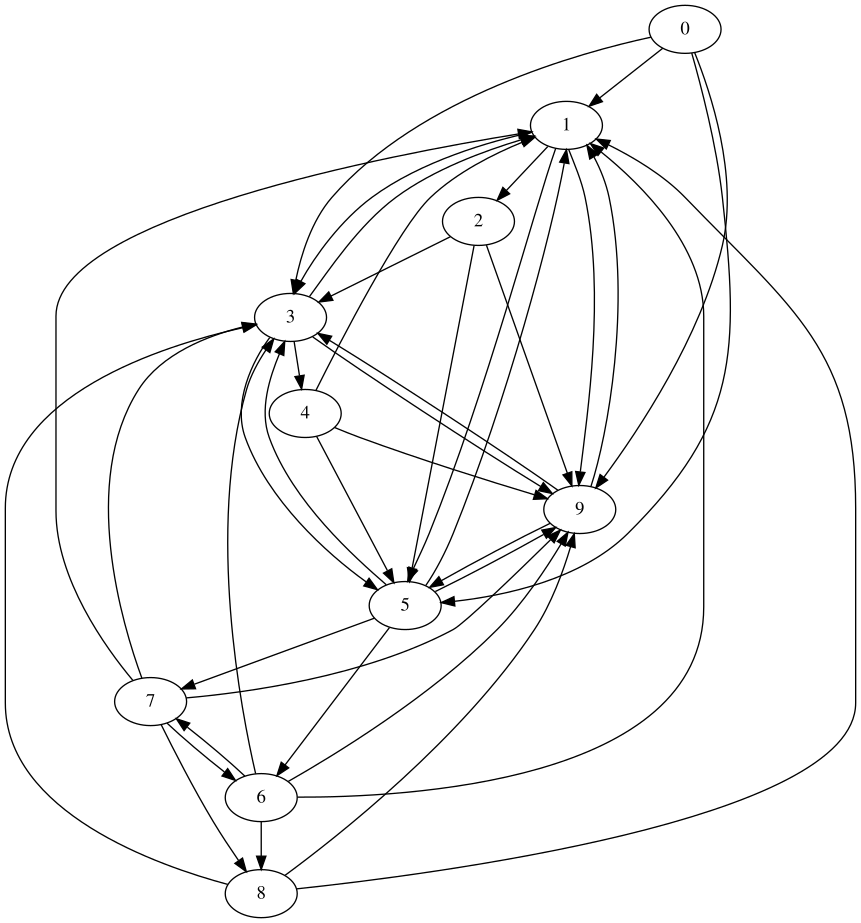
\includegraphics[width=0.8\textwidth]{title_graph.png}
}
\author{Richèl J.C. Bilderbeek}

% Use double spacing
\usepackage{setspace}
\doublespacing

\usepackage{listings}
\usepackage{hyperref}
\usepackage{todonotes}
\usepackage{verbatim}
\usepackage{pgf}
\usepackage{bm}
\usepackage{multirow}
\usepackage{amsfonts}
\usepackage{array}
\usepackage{booktabs}
\newcolumntype{C}[1]{>{\centering\arraybackslash}p{#1}}
\newcolumntype{L}[1]{>{\raggedright\arraybackslash}p{#1}}
\usepackage{longtable}

% sidewaysfigure
\usepackage{rotating}

% Style of listings
% From http://r.789695.n4.nabble.com/
%   How-to-nicely-display-R-code-with-the-LaTeX-package-listings-tp4648110.html
\usepackage{fancyvrb} 
\definecolor{codegreen}{rgb}{0,0.6,0}
\definecolor{codegray}{rgb}{0.5,0.5,0.5}
\definecolor{codepurple}{rgb}{0.58,0,0.82}
\definecolor{backcolor}{rgb}{0.95,0.95,0.92}
\lstdefinestyle{mystyle}{
  language=R,% set programming language
  basicstyle=\ttfamily\small,% basic font style
  commentstyle=\color{gray},% comment style
  numberstyle=\scriptsize,% use small line numbers
  numbersep=10pt,% space between line numbers and code
  tabsize=2,% sizes of tabs
  showstringspaces=false,
  captionpos=b,% positioning of the caption below
  breaklines=true,% automatic line breaking
  escapeinside={(*}{*)},% escaping to LaTeX
  fancyvrb=true,% verbatim code is typset by listings
  extendedchars=false,% prohibit extended chars (chars of codes 128--255)
  alsoletter={.<-},% becomes a letter
  alsoother={$},% becomes other
  otherkeywords={!=, ~, $, \&, \%/\%, \%*\%, \%\%, <-, <<-, /},
  deletekeywords={c}% remove keywords 
}
\lstset{style=mystyle}

% Adds numbered lines
% \usepackage{lineno}
% \linenumbers

% Subfigures
\usepackage{subcaption}

% Subfigure numbers use uppercase, 
% from https://tex.stackexchange.com/a/278140
\renewcommand{\thesubfigure}{\Alph{subfigure}}

\begin{document}

\maketitle

%\begin{figure}[!h]
%  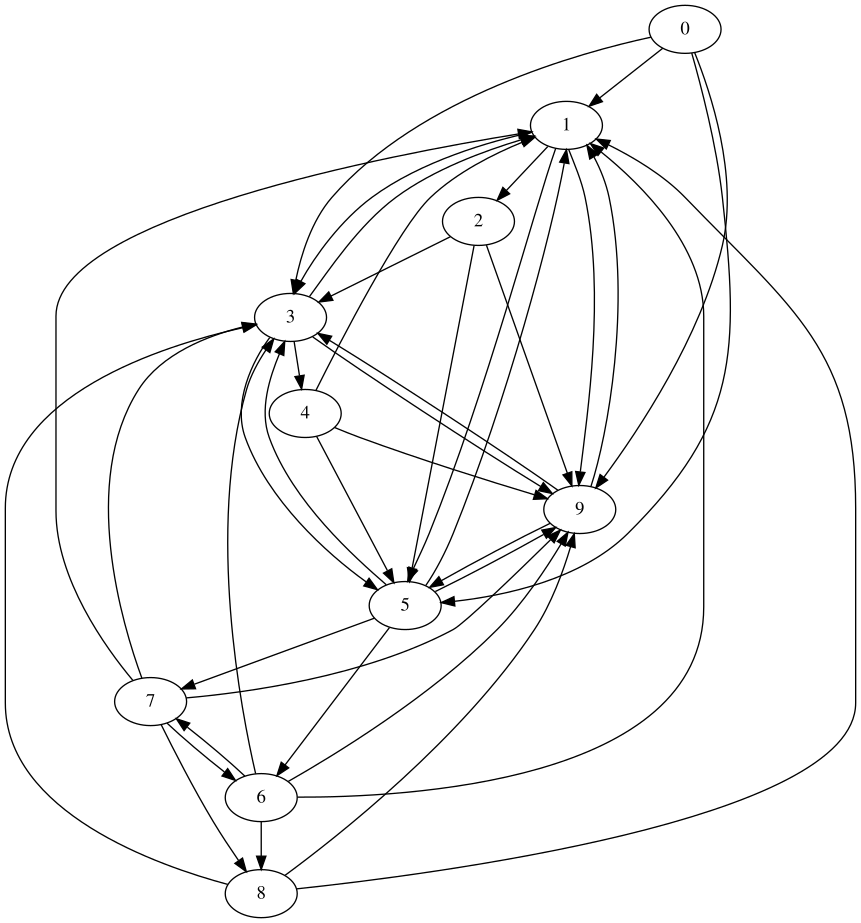
\includegraphics[width=0.4\textwidth]{title_graph.png}
%  \label{fig:title}
%\end{figure}

%%%%%%%%%%%%%%%%%%%%%%%%%%%%%%%%%%%%%%%%%%%%%%%%%%%%%%%%%%%%%%%%%%%%%%%%%%%%%%%%%
\chapter{Introduction}
%%%%%%%%%%%%%%%%%%%%%%%%%%%%%%%%%%%%%%%%%%%%%%%%%%%%%%%%%%%%%%%%%%%%%%%%%%%%%%%%

This is 'Boost.Graph Cookbook 1: Basics', version 3.3.

\subsection{Why this tutorial}

I needed this tutorial already in 2006, when I started experimenting with
Boost.Graph.
More specifically, I needed a tutorial that:

\begin{itemize}
  \item Orders concepts chronologically
  \item Increases complexity gradually
  \item Shows complete pieces of code
\end{itemize}

What I had were the book \cite{siek2001boost}
and the Boost.Graph website, both did not satisfy these requirements.

\subsection{Tutorial style}

\paragraph{Readable for beginners}

This tutorial is aimed at the beginner programmer.
This tutorial is intended to take the reader to the level of understanding
the book \cite{siek2001boost}
and the Boost.Graph website require.
It is about basic graph manipulation, not the more advanced graph algorithms.
 
\paragraph{High verbosity}

This tutorial is intended to be as verbose, such that a beginner should
be able to follow every step, from reading the tutorial from beginning
to end chronologically.
Especially in the earlier chapters, the rationale behind the code presented
is given, including references to the literature.
Chapters marked with $\triangle$ are optional, 
less verbose and bring no new information to the storyline.

\paragraph{Repetitiveness}

This tutorial is intended to be as repetitive, such that a beginner can
 spot the patterns in the code snippets their increasing complexity.
 Extending code from this tutorial should be as easy as extending the patterns.

\paragraph{Index}

In the index, I did first put all my long-named functions there literally,
but this resulted in a very sloppy layout.
Instead, the function 'do\_something' can be found as 'Do something' in
the index.
On the other hand, STL and Boost functions like 'std::do\_something' and
'boost::do\_something' can be found as such in the index.

\subsection{Coding style}

\paragraph{Concept}

For every concept, I will show

\begin{itemize}
    \item a function that achieves a goal, 
      for example \verb;create_empty_undirected_graph;
    \item{
      a test case of that function, 
      that demonstrates how to use the function, for example
      \verb;create_empty_undirected_graph_test;
    }
    \item Three
\end{itemize}

\paragraph{C++14}

All coding snippets are taken from compiled and tested C++14 code.
I chose to use C++14 because it was available to me on all local and remote
computers.
Next to this, it makes code even shorter then just C++11.

\paragraph{Coding standard}

I use the coding style from the Core C++ Guidelines.
At the time of this writing, the Core C++ Guidelines were still in early
development, so I can only hope the conventions I then chose to follow
are still Good Ideas.

\paragraph{No comments in code}

It is important to add comments to code.
In this tutorial, however, I have chosen not to put comments in code, as
I already describe the function in the tutorial its text.
This way, it prevents me from saying the same things twice.

\paragraph{Trade-off between generic code and readability}

It is good to write generic code.
In this tutorial, however, I have chosen my functions to have no templated
arguments for conciseness and readability.
For example, a vertex name is std::string, the type for if a vertex is
selected is a boolean, and the custom vertex type is of type \verb;my_custom_vertex;.
I think these choices are reasonable and that the resulting increase in
readability is worth it.

\paragraph{Long function names}

I enjoy to show concepts by putting those in (long-named) functions.
These functions sometimes border the trivial, by, for example, only calling
a single Boost.Graph function.
On the other hand, these functions have more English-sounding names, resulting
in demonstration code that is readable.
Additionally, they explicitly mention their return type (in a simpler way),
which may be considered informative.

\paragraph{Long function names and readability}

Due to my long function names and the limitation of ≈50 characters per line,
sometimes the code does get to look a bit awkward.
I am sorry for this.

\paragraph{Use of auto}

I prefer to use the keyword auto over doubling the lines of code for using
statements.
Often the \verb;do; functions return an explicit data type, these can be used
for reference.
Sometime I deduce the return type using decltype and a function with the
same return type.
When C++17 gets accessible, I will use \verb;decltype(auto);
If you really want to know a type, you can use the \verb;get_type_name; function
(chapter \ref{subsec:get_type_name})

\subparagraph{Explicit use of namespaces}

On the other hand, I am explicit in the namespaces of functions and classes
I use, so to distinguish between types like \verb;std::array; and \verb;boost::array;.
Some functions (for example, \verb;get;) reside 
in the namespace of the graph to work on.
In this tutorial, this is in the global namespace.
Thus, I will write \verb;get;, instead of \verb;boost::get;, 
as the latter does not compile.

\paragraph{Use of STL algorithms}

I try to use STL algorithms wherever I can.
Also you should prefer algorithm calls over hand-written 
for-loops (\cite{stroustrup1997}, chapter 18.12.1 and \cite{meyers2005effective}, item 43).
Sometimes using these algorithms becomes a burden on the lines of code.
This is because in C++11, a lambda function argument (use by the algorithm)
must have its data type specified.
It may take multiple lines of \verb;using; statements being able to do so.
In C++14 one can use \verb;auto; there as well.
So, only if it shortens the number of lines significantly, I use raw for-loops,
even though you shouldn't.

\paragraph{Re-use of functions}

The functions I develop in this tutorial are re-used from that moment on.
This improves to readability of the code and decreases the number of lines.

\paragraph{Tested to compile}

All functions in this tutorial are tested to compile using GitHub Actions in
both debug and release mode.

\paragraph{Tested to work}

All functions in this tutorial are tested, using the Boost.Test library.
GitHub Actions calls these tests after each push to the repository.

\paragraph{Availability}

The code, as well as this tutorial, can be downloaded from the GitHub at
\url{www.github.com/richelbilderbeek/boost_graph_cookbook_1}.

\subsection{License}

This tutorial is licensed under Creative Commons license 4.0.
All C++ code is licensed under GPL 3.0.

\begin{figure}[!htbp]
  
\includegraphics[]{CC-BY-SA_icon.png}
  \caption{
    Creative Commons license 4.0
  }
  \label{fig:license}
\end{figure}

\subsection{Feedback}

This tutorial is not intended to be perfect yet.
For that, I need help and feedback from the community.
All referenced feedback is welcome, as well as any constructive feedback.

I have tried hard to strictly follow the style as described above.
If you find I deviated from these decisions somewhere, I would be grateful
if you'd let know.
Next to this, there are some sections that need to be coded or have its
code improved.

\subsection{Acknowledgements}


These are users that improved this tutorial and/or the code behind this
tutorial, in chronological order:

\begin{itemize}
  \item m-dudley, \url{http://stackoverflow.com/users/111327/m-dudley}
  \item E. Kawashima
  \item mat69, \url{https://www.reddit.com/user/mat69}
  \item danielhj, \url{https://www.reddit.com/user/danieljh}
  \item sehe, \url{http://stackoverflow.com/users/85371/sehe}
  \item cv\_and\_me, \url{http://stackoverflow.com/users/2417774/cv-and-he}
  \item mywtfmp3
\end{itemize}

\subsection{Outline}

The chapters of this tutorial are also like a well-connected graph.
To allow for quicker learners to skim chapters, or for beginners looking
to find the patterns.

The distinction between the chapter is in the type of edges and vertices.
They can have:

\begin{itemize}
  \item no properties: 
    see chapter \ref{sec:Building-graphs-without-properties}
  \item have a bundled property: 
    see chapter \ref{sec:Building-graphs-with-bundled-vertices}
\end{itemize}

Pivotal chapters are chapters like 'Finding the first vertex with ...', as
this opens up the door to finding a vertex and manipulating it.

All chapters have a rather similar structure in themselves, as depicted
in figure \ref{fig:The-relations-between-subchapters}.

\begin{figure}[!htbp]
  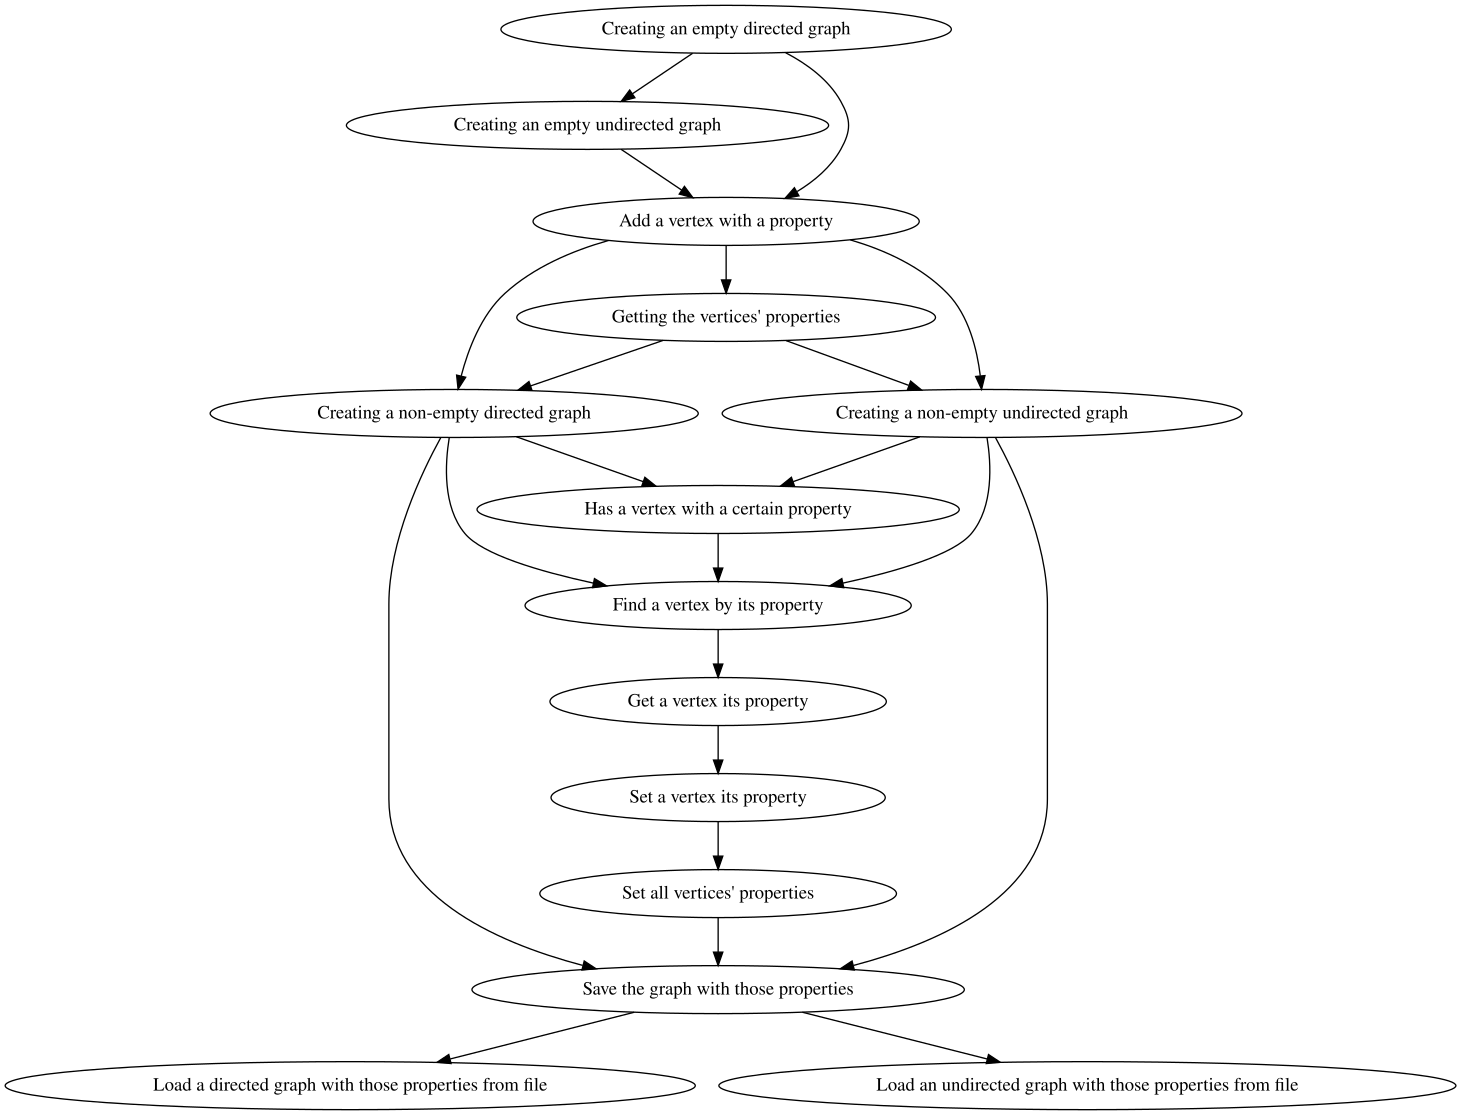
\includegraphics[width=\textwidth]{create_tutorial_subchapters_graph.png}
  \caption{
    The relations between sub-chapters
  }
  \label{fig:The-relations-between-subchapters}
\end{figure}

There are also some bonus chapters, that I have labeled with a $\triangle$.
These chapters are added I needed these functions myself and adding them
would not hurt.
Just feel free to skip them, as there will be less theory explained.


%%%%%%%%%%%%%%%%%%%%%%%%%%%%%%%%%%%%%%%%%%%%%%%%%%%%%%%%%%%%%%%%%%%%%%%%%%%%%%%%%
\chapter{Building graphs without properties}
\label{sec:Building-graphs-without-properties}
%%%%%%%%%%%%%%%%%%%%%%%%%%%%%%%%%%%%%%%%%%%%%%%%%%%%%%%%%%%%%%%%%%%%%%%%%%%%%%%%

Boost.Graph is about creating graphs.
In this chapter we create the simplest of graphs, in which edges and nodes
have no properties (e.g. having a name).

Still, there are two types of graphs that can be constructed: undirected
and directed graphs.
The difference between directed and undirected graphs is in the edges:
in an undirected graph, 
an edge connects two vertices without any directionality, as displayed
in figure \ref{fig:undirected_graph_example}.

In a directed graph, an edge goes from a certain vertex, 
its source, to another (which may actually be the same), its target.
A directed graph is shown in figure \ref{fig:directed_graph_example}.

\begin{figure}
  \begin{tikzpicture}
    \draw[thick] 
      (0,0) node[draw=black,fill=white,shape=circle,text=white] {} 
      -- (5,2) node[draw=black,fill=white,shape=circle,text=white] {} 
      -- (10,1) node[draw=black,fill=white,shape=circle,text=white] {} 
    ;
  \end{tikzpicture}
  \caption{Example of an undirected graph}
  \label{fig:undirected_graph_example}
\end{figure}

\begin{figure}
  \begin{tikzpicture}
    \SetGraphUnit{5}
    \tikzset{VertexStyle/.append style = {draw=black,fill=white,shape=circle,text=white} }
    \Vertex{A}
    \EA(A){B}
    \EA(B){C}
    \tikzset{EdgeStyle/.append style = {->, bend left} }
    \Edge[](A)(B)
    \Edge[](B)(A)
    \Loop[dist = 4cm, dir = NO](A.west)
    \tikzset{EdgeStyle/.append style = {bend left = 0} }
    \Edge[](C)(B)   
  \end{tikzpicture}
  \caption{Example of a directed graph}
  \label{fig:directed_graph_example}
\end{figure}

In this chapter, we will build two directed and two undirected graphs:

\begin{itemize}
  \item An empty (directed) graph, which is the default type: 
    see chapter \ref{subsec:create_empty_directed_graph}
  \item An empty (undirected) graph: 
    see chapter \ref{subsec:create_empty_undirected_graph}
  \item A two-state Markov chain, a directed graph with two vertices 
    and four edges:
    see chapter \ref{subsec:create_markov_chain_graph}
  \item $K_{2}$, an undirected graph with two vertices and one edge, 
    see chapter \ref{subsec:create_k2_graph}
\end{itemize}


Creating an empty graph may sound trivial, it is not, thanks to the versatility
of the Boost.Graph library.

In the process of creating graphs, some basic (sometimes bordering trivial)
functions are encountered:

\begin{itemize}
  \item Counting the number of vertices, 
    see chapter \ref{subsec:get_n_vertices}
  \item Counting the number of edges,
     see chapter \ref{subsec:get_n_edges}
  \item Adding a vertex,
     see chapter \ref{subsec:add_vertex}
  \item Getting all vertices,
     see chapter \ref{subsec:get_vertices}
  \item Getting all vertex descriptors,
     see chapter \ref{subsec:get_vertex_descriptors}
  \item Adding an edge,
     see chapter \ref{subsec:add_edge}
  \item Getting all edges,
    see chapter \ref{subsec:get_edge_iterators}
  \item Getting all edge descriptors,
    see chapter \ref{subsec:get_edge_descriptors}
\end{itemize}

These functions are mostly there for completion and showing which data types
are used.

The chapter also introduces some important concepts:

\begin{itemize}
  \item Vertex descriptors,
    see chapter \ref{subsec:Vertex-descriptors}
  \item Edge insertion result,
    see chapter \ref{subsec:add_edge}
  \item Edge descriptors,
    see chapter \ref{subsec:Edge-descriptors}
\end{itemize}

After this chapter you may want to:

\begin{itemize}
  \item Building graphs with named vertices, 
    see chapter \ref{sec:Building-graphs-with-named-vertices}
  \item Building graphs with bundled vertices, 
    see chapter \ref{sec:Building-graphs-with-bundled-vertices}
  \item Building graphs with custom vertices,
    see chapter \ref{sec:Building-graphs-with-custom-properties}
  \item Building graphs with a graph name,
    see chapter \ref{sec:Building-graphs-with-a-graph-name}
\end{itemize}

%%%%%%%%%%%%%%%%%%%%%%%%%%%%%%%%%%%%%%%%%%%%%%%%%%%%%%%%%%%%%%%%%%%%%%%%%%%%%%%%
\subsection{Creating an empty (directed) graph}
\label{subsec:create_empty_directed_graph}
%%%%%%%%%%%%%%%%%%%%%%%%%%%%%%%%%%%%%%%%%%%%%%%%%%%%%%%%%%%%%%%%%%%%%%%%%%%%%%%%

Let's create an empty graph! 
Listing \ref{lst:create_empty_directed_graph} 
shows the function to create an empty graph.

\lstinputlisting[
  caption = Creating an empty (directed) graph,
  label = lst:create_empty_directed_graph
]{create_empty_directed_graph.impl}

The code consists out of an \verb;#include; and a function definition.
The \verb;#include; tells the compiler 
to read the header file \verb;adjacency_list.hpp;.
A header file (often with a \verb;.h; or \verb;.hpp; extension) 
contains class and functions declarations and/or definitions.
The header file \verb;adjacency_list.hpp; contains the 
\verb;boost::adjacency_list; class definition.
Without including this file, you will get compile errors like 
\verb;definition of boost::adjacency_list; unknown;
\footnote{
  In practice, these compiler error messages will be longer, bordering the unreadable
}. 

The function \verb;create_empty_directed_graph; has:

\begin{itemize}
  \item a return type: 
    The return type is \verb;boost::adjacency_list<>;, 
    that is a \verb;boost::adjacency_list; 
    with all template arguments set at their defaults
  \item a \verb;noexcept; specification: 
    the function should not throw
    \footnote{
      if the function would throw because it cannot allocate this little piece
      of memory, you are already in big trouble
    }, so it is preferred to mark it \verb;noexcept; 
    (\cite{stroustrup2013}, chapter 13.7)
  \item a function body: 
    all the function body does is implicitly create its return
    type by using the \verb;{};.
    An alternative syntax would be \verb;return boost::adjacency_list<>();,
    which is needlessly longer
\end{itemize}

Listing \ref{lst:create_empty_directed_graph_demo}
demonstrates the \verb;create_empty_directed_graph; function.
This demonstration is embedded within a Boost.Test unit test case.
It includes a Boost.Test header to allow to use the Boost.Test framework.
Additionally, a header file is included with the same name as the function
\footnote{
  I do not think it is important to have creative names
}.
This allows use to be able to use the function.
The test case creates an empty graph and stores it.
Instead of specifying the data type explicitly, 
\verb;auto; \index{auto} is used (this is preferred, \cite{stroustrup2013}
chapter 31.6), which lets the compiler figure out the type itself.

\lstinputlisting[
  caption = Demonstration of create\_empty\_directed\_graph,
  label = lst:create_empty_directed_graph_demo
]{create_empty_directed_graph_demo.impl}

Congratulations, you've just created a 
\verb;boost::adjacency_list; \index{boost::adjacency\_list}
with its default template arguments.
The \verb;boost::adjacency_list; is the most commonly used graph type, the other
is the \verb;boost::adjacency_matrix; \index{boost::adjacency\_matrix}.

We do not do anything with it yet, but still, you've just created a graph,
in which:

\begin{itemize}
  \item The out edges and vertices are stored in a \verb;std::vector; \index{std::vector}
  \item The edges have a direction
  \item The vertices, edges and graph have no properties
  \item The edges are stored in a \verb;std::list; \index{std::list}
\end{itemize}

It stores its edges, out edges and vertices in two different STL \index{STL}
\footnote{
  Standard Template Library, the standard library
}
containers.
std::vector \index{std::vector} is the container you should use by default (
  \cite{stroustrup2013}, chapter 31.6, 
  \cite{sutter_and_alexandrescu2004}, chapter 76
), as it has constant time look-up and back insertion.
The \verb;std::list; \index{std::list}
is used for storing the edges, as it is better suited at inserting elements
at any position.

I use \verb;const; \index{const} to store the empty graph as we do not modify it.
Correct use of \verb;const; is called const-correct.
Prefer to be const-correct \index{const-correctness}
(
  \cite{stroustrup1997}, chapter 7.9.3, 
  \cite{stroustrup2013}, chapter 12.7, 
  \cite{meyers2005effective}, item 3, 
  \cite{hollingworth2000cpp_builder_dev_guide}, chapter 3, 
  \cite{sutter_and_alexandrescu2004}, item 15, 
  \cite{cline1998cpp_faqs}, FAQ 14.05, 
  \cite{eckel2002thinking_cpp}, item 8, 
  \cite{lakos1996large}, 9.1.6
).

%%%%%%%%%%%%%%%%%%%%%%%%%%%%%%%%%%%%%%%%%%%%%%%%%%%%%%%%%%%%%%%%%%%%%%%%%%%%%%%%
\subsection{Creating an empty undirected graph}
\label{subsec:create_empty_undirected_graph}
\index{Create an empty graph}
\index{Empty graph, create}
\index{Create empty undirected graph}
%%%%%%%%%%%%%%%%%%%%%%%%%%%%%%%%%%%%%%%%%%%%%%%%%%%%%%%%%%%%%%%%%%%%%%%%%%%%%%%%

Let's create another empty graph! This time, we even make it undirected!
Listing \ref{lst:create_empty_undirected_graph}
shows how to create an undirected graph.

\lstinputlisting[
  caption = Creating an empty undirected graph,
  label = lst:create_empty_undirected_graph
]{create_empty_undirected_graph.impl}

This algorithm differs from the \verb;create_empty_directed_graph;
function (algorithm 
\ref{lst:create_empty_directed_graph}
) 
in that there are three template arguments that need to be specified in
the creation of the \verb;boost::adjacency_list;:

\begin{itemize}
  \item the first \verb;boost::vecS; \index{boost::vecS}: 
    select (that is what the \verb;S; \index{S}
    means) that out edges are stored in a std::vector.
    This is the default way.
  \item
    the second \verb;boost::vecS; \index{boost::vecS}: 
    select that the graph vertices are stored in a std::vector.
    This is the default way.
  \item
    \verb;boost::undirectedS; \index{boost::undirectedS}: 
    select that the graph is undirected.
    This is all we needed to change.
    By default, this argument is boost::directed \index{boost::directedS}
\end{itemize}

Listing \ref{lst:create_empty_undirected_graph_demo}
demonstrates the \verb;create_empty_undirected_graph; function.

\lstinputlisting[
  caption = Demonstration of create\_empty\_undirected\_graph,
  label = lst:create_empty_undirected_graph_demo
]{create_empty_undirected_graph_demo.impl}

Congratulations, with algorithm \ref{lst:create_empty_undirected_graph_demo}, 
you have just created an undirected graph in which:

\begin{itemize}
  \item The out edges and vertices are stored in a std::vector
  \item The graph is undirected
  \item Vertices, edges and graph have no properties
  \item Edges are stored in a std::list
\end{itemize}

%%%%%%%%%%%%%%%%%%%%%%%%%%%%%%%%%%%%%%%%%%%%%%%%%%%%%%%%%%%%%%%%%%%%%%%%%%%%%%%%
\subsection{Counting the number of vertices}
\label{subsec:get_n_vertices}
\index{Vertices, counting}
\index{Counting the number of vertices}
\index{Number of vertices, get}
\index{Get n vertices}
%%%%%%%%%%%%%%%%%%%%%%%%%%%%%%%%%%%%%%%%%%%%%%%%%%%%%%%%%%%%%%%%%%%%%%%%%%%%%%%%

Let's count all zero vertices of an empty graph!

\lstinputlisting[
  caption = Count the number of vertices,
  label = lst:get_n_vertices
]{get_n_vertices.impl}

The function \verb;get_n_vertices; takes the result of \verb;boost::num_vertices;
\index{boost::num\_vertices}, converts it to int and checks if there was conversion error.
We do so, as one should prefer using signed data types over unsigned ones
in an interface (\cite{lakos1996large}, chapter 9.2.2).
To do so, in the function body its first statement, 
the unsigned long \index{unsigned long}
produced by \verb;boost::num_vertices; \index{boost::num\_vertices}
get converted to an int using a \verb;static_cast; \index{static\_cast}.

Using an unsigned integer over a (signed) integer for the sake of gaining
that one more bit (\cite{stroustrup1997}, chapter 4.4) should be avoided.
The integer \verb;n; is initialized using list-initialization, which is preferred
over the other initialization syntaxes (\cite{stroustrup2013}, chapter 17.7.6).

The \verb;assert; checks if the conversion back to unsigned long re-creates the
original value, to check if no information has been lost.
If information is lost, the program crashes.
Use \verb;assert; \index{assert} extensively 
(\cite{stroustrup1997}, chapter 24.5.18, 
\cite{stroustrup2013}, chapter 30.5, 
\cite{sutter_and_alexandrescu2004}. chapter 68, 
\cite{mcconnell2004code}, chapter 8.2, 
\cite{liberty2001sams}, hour 24, 
\cite{lakos1996large}, chapter 2.6).

The function \verb;get_n_vertices; is demonstrated in algorithm 
\ref{lst:get_n_vertices_demo}, 
to measure the number of vertices of both the directed and undirected
graph we are already able to create.

\lstinputlisting[
  caption = Demonstration of the get\_n\_vertices function,
  label = lst:get_n_vertices_demo
]{get_n_vertices_demo.impl}

Note that the type of graph does not matter here.
One can count the number of vertices of every graph, as all graphs have
vertices.
Boost.Graph is very good at detecting operations that are not allowed, during
compile time.

%%%%%%%%%%%%%%%%%%%%%%%%%%%%%%%%%%%%%%%%%%%%%%%%%%%%%%%%%%%%%%%%%%%%%%%%%%%%%%%%
\subsection{Counting the number of edges}
\label{subsec:get_n_edges}
\index{Edges, counting}
\index{Counting the number of edges}
\index{Number of edges, get}
\index{Get n edges}
%%%%%%%%%%%%%%%%%%%%%%%%%%%%%%%%%%%%%%%%%%%%%%%%%%%%%%%%%%%%%%%%%%%%%%%%%%%%%%%%

Let's count all zero edges of an empty graph!

This is very similar to the previous chapter, 
only it uses \verb;boost::num_edges; \index{boost::num\_edges}
instead:

\lstinputlisting[
  caption = Count the number of edges,
  label = lst:get_n_edges
]{get_n_edges.impl}

This code is similar to the \verb;get_n_vertices; 
function (algorithm \ref{lst:get_n_vertices}, see rationale there) 
except \verb;boost::num_edges; \index{boost::num\_edges}
is used, instead of \verb;boost::num_vertices;, 
which also returns an unsigned long.

The function \verb;get_n_edges; is demonstrated in algorithm 
\ref{lst:get_n_edges_demo}, 
to measure the number of edges of an empty directed and undirected graph.

\lstinputlisting[
  caption = Demonstration of the get\_n\_edges function,
  label = lst:get_n_edges_demo
]{get_n_edges_demo.impl}

%%%%%%%%%%%%%%%%%%%%%%%%%%%%%%%%%%%%%%%%%%%%%%%%%%%%%%%%%%%%%%%%%%%%%%%%%%%%%%%%
\subsection{Adding a vertex}
\label{subsec:add_vertex}
\index{Add a vertex}
\index{Vertex, add}
\index{Add vertex}
%%%%%%%%%%%%%%%%%%%%%%%%%%%%%%%%%%%%%%%%%%%%%%%%%%%%%%%%%%%%%%%%%%%%%%%%%%%%%%%%

Empty graphs are nice, now its time to add a vertex!

To add a vertex to a graph, 
the \verb;boost::add_vertex; \index{boost::add\_vertex}
function is used as shows in algorithm \ref{lst:add_vertex}:

\lstinputlisting[
  caption = Adding a vertex to a graph,
  label = lst:add_vertex
]{add_vertex.impl}

The \verb;static_assert; \index{static\_assert}
at the top of the function checks during compiling if the function is called
with a non-const graph.
One can freely omit this \verb;static_assert;: you will get a compiler error anyways,
be it a less helpful one.

Note that \verb;boost::add_vertex; (in the \verb;add_vertex; function) 
returns a vertex
descriptor, which is ignored for now.
Vertex descriptors are looked at in more details 
at the chapter \ref{subsec:Vertex-descriptors}, 
as we need these to add an edge.
To allow for this already, \verb;add_vertex; also returns a vertex descriptor.

Listing \ref{lst:add_vertex_demo}
shows how to add a vertex to a directed and undirected graph.

\lstinputlisting[
  caption = Demonstration of the add\_vertex function,
  label = lst:add_vertex_demo
]{add_vertex_demo.impl}

This demonstration code creates two empty graphs, adds one vertex to each
and then \verb;assert;s that the number of vertices in each graph is one.
This works for both types of graphs, as all graphs have vertices.

%%%%%%%%%%%%%%%%%%%%%%%%%%%%%%%%%%%%%%%%%%%%%%%%%%%%%%%%%%%%%%%%%%%%%%%%%%%%%%%%
\subsection{Vertex descriptors}
\label{subsec:Vertex-descriptors}
\index{Vertex descriptor}
%%%%%%%%%%%%%%%%%%%%%%%%%%%%%%%%%%%%%%%%%%%%%%%%%%%%%%%%%%%%%%%%%%%%%%%%%%%%%%%%

A vertex descriptor is a handle to a vertex within a graph.

Vertex descriptors can be obtained by dereferencing a vertex iterator (see
chapter \ref{subsec:get_vertex_descriptors}).
To do so, we first obtain some vertex iterators in chapter 
\ref{subsec:get_vertices}).
 
Vertex descriptors are used to:

\begin{itemize}
  \item add an edge between two vertices, see chapter \ref{subsec:add_edge}
  \item obtain properties of vertex a vertex, 
    for example the vertex its out degrees (chapter \ref{subsec:get_vertex_out_degrees}), 
    the vertex its name (chapter \ref{subsec:get_vertex_names}), 
    or a custom vertex property (chapter \ref{subsec:get_vertex_my_vertexes})
\end{itemize}

In this tutorial, 
vertex descriptors have named prefixed with \verb;vd_; \index{vd\_}, 
for example \verb;vd_1;.

%%%%%%%%%%%%%%%%%%%%%%%%%%%%%%%%%%%%%%%%%%%%%%%%%%%%%%%%%%%%%%%%%%%%%%%%%%%%%%%%
\subsection{}
Get the vertex iterators
\label{subsec:get_vertices}
\index{Vertex iterator}
\index{Vertex iterators, get}
\index{Get vertex iterators}
\index{Get vertices}
%%%%%%%%%%%%%%%%%%%%%%%%%%%%%%%%%%%%%%%%%%%%%%%%%%%%%%%%%%%%%%%%%%%%%%%%%%%%%%%%

You cannot get the vertices.
This may sound unexpected, as it must be possible to work on the vertices
of a graph.
Working on the vertices of a graph is done through these steps:

\begin{itemize}
  \item Obtain a vertex iterator pair from the graph
  \item Dereferencing a vertex iterator to obtain a vertex descriptor 
\end{itemize}

\verb;vertices; \index{vertices} 
(not \verb;boost::vertices; \index{boost::vertices does not exist}) 
is used to obtain 
a vertex iterator pair \index{Vertex iterator pair}, 
as shown in algorithm \ref{lst:get_vertex_iterators}.

The first vertex iterator \index{Vertex iterator}
points to the first vertex (its descriptor, to be precise), the second
points to beyond the last vertex (its descriptor, to be precise).
In this tutorial, vertex iterator pairs have named prefixed with 
\verb;vip_; \index{vip\_}, for example \verb;vip_1;.

\lstinputlisting[
  caption = Get the vertex iterators of a graph,
  label = lst:get_vertex_iterators
]{get_vertex_iterators.impl}

This is a somewhat trivial function, 
as it forwards the function call to
\verb;vertices; \index{vertices}
(not \verb;boost::vertices; \index{boost::vertices does not exist}).

These vertex iterators can be dereferenced to obtain the vertex descriptors.
Note that \verb;get_vertex_iterators; will not be used often in isolation: usually
one obtains the vertex descriptors immediately.
Just for your reference, algorithm 
\ref{lst:get_vertex_iterators_demo}
demonstrates of the \verb;get_vertices; function, by showing that the vertex
iterators of an empty graph point to the same location.

\lstinputlisting[
  caption = Demonstration of get\_vertex\_iterators,
  label = lst:get_vertex_iterators_demo
]{get_vertex_iterators_demo.impl}

%%%%%%%%%%%%%%%%%%%%%%%%%%%%%%%%%%%%%%%%%%%%%%%%%%%%%%%%%%%%%%%%%%%%%%%%%%%%%%%%
\subsection{Get all vertex descriptors}
\label{subsec:get_vertex_descriptors}
\index{Vertex descriptors, get}
\index{Get vertex descriptors}
%%%%%%%%%%%%%%%%%%%%%%%%%%%%%%%%%%%%%%%%%%%%%%%%%%%%%%%%%%%%%%%%%%%%%%%%%%%%%%%%

Vertex descriptors are the way to manipulate those vertices.
Let's go get the all!

Vertex descriptors are obtained from dereferencing vertex iterators.
Listing \ref{lst:get_vertex_descriptors}
shows how to obtain all vertex descriptors from a graph.

\lstinputlisting[
  caption = Get all vertex descriptors of a graph,
  label = lst:get_vertex_descriptors
]{get_vertex_descriptors.impl}

This is the first more complex piece of code.
In the first lines, some \verb;using; statements allow for shorter type names
\footnote{
  which may be necessary just to create a tutorial 
  with code snippets that are readable
}.

The std::vector to serve as a return value is created at the needed size,
which is the number of vertices.

The function \verb;vertices; \index{vertices}

(not boost::vertices \index{boost::vertices does not exist}!) 
returns a vertex iterator pair.
These iterators are used by std::copy to iterator over.
std::copy \index{std::copy}
is an STL algorithm to copy a half-open range.
Prefer algorithm calls over hand-written for-loops (
\cite{stroustrup1997} chapter 18.12.1, 
\cite{meyers2005effective} item 43).
In this case, we copy all vertex descriptors in the range produced 
by \verb;vertices; to the std::vector.

This function will not be used in practice: one iterates over the vertices
directly instead, saving the cost of creating a std::vector.
This function is only shown as an illustration.

Listing \ref{lst:get_vertex_descriptors_demo}
demonstrates that an empty graph has no vertex descriptors:

\lstinputlisting[
  caption = Demonstration of get\_vertex\_descriptors,
  label = lst:get_vertex_descriptors_demo
]{get_vertex_descriptors_demo.impl}

Because all graphs have vertices and thus vertex descriptors, the type of
graph is unimportant for this code to compile.

%%%%%%%%%%%%%%%%%%%%%%%%%%%%%%%%%%%%%%%%%%%%%%%%%%%%%%%%%%%%%%%%%%%%%%%%%%%%%%%%
\subsection{Add an edge}
\label{subsec:add_edge}
\index{Add an edge}
\index{Edge, add}
%%%%%%%%%%%%%%%%%%%%%%%%%%%%%%%%%%%%%%%%%%%%%%%%%%%%%%%%%%%%%%%%%%%%%%%%%%%%%%%%

To add an edge to a graph, two vertex descriptors are needed.
A vertex descriptor \index{Vertex descriptor}
is a handle to the vertex within a graph (vertex descriptors are looked
 at in more details in chapter 
\ref{subsec:Vertex-descriptors}).
Listing \ref{lst:add_edge}
adds two vertices to a graph, and connects these two using 
\verb;boost::add_edge; \index{boost::add\_edge}: 

\lstinputlisting[
  caption = Adding (two vertices and) an edge to a graph,
  label = lst:add_edge
]{add_edge.impl}

Listing \ref{lst:add_edge}

shows how to add an isolated edge to a graph (instead of allowing for graphs
with higher connectivities).
First, two vertices are created, using the function \verb;boost::add_vertex;.
\verb;boost::add_vertex; returns a vertex descriptor 
(which I prefix with \verb;vd; \index{vd}), 
both of which are stored.
The vertex descriptors are used to add an edge to the graph, 
using 
\verb;boost::add_edge; \index{boost::add\_edge}.

\verb;boost::add_edge; \index{boost::add\_edge}
returns a std::pair \index{std::pair}, 
consisting of an edge descriptor and a boolean success indicator.
The success of adding the edge is checked by an \verb;assert; statement.
Here we \verb;assert; \index{assert}
that this insertion was successful.
Insertion can fail if an edge is already present and duplicates are not
allowed.

A demonstration of \verb;add_edge; is shown in algorithm 
\ref{lst:add_edge_demo}, 
in which an edge is added to both a directed and undirected graph, 
after which the number of edges and vertices is checked.

\lstinputlisting[
  caption = Demonstration of add\_edge,
  label = lst:add_edge_demo
]{add_edge_demo.impl}

The graph type is unimportant: as all graph types have vertices and edges,
 edges can be added without possible compile problems.

%%%%%%%%%%%%%%%%%%%%%%%%%%%%%%%%%%%%%%%%%%%%%%%%%%%%%%%%%%%%%%%%%%%%%%%%%%%%%%%%
\subsection{boost::add_edge result}
\label{subsec:boost_add_edge_result}
\index{boost::add\_edge result}
%%%%%%%%%%%%%%%%%%%%%%%%%%%%%%%%%%%%%%%%%%%%%%%%%%%%%%%%%%%%%%%%%%%%%%%%%%%%%%%%

When using the function \verb;boost::add_edge;, 
a \verb;std::pair<edge_descriptor,bool>; is returned.
It contains both the edge descriptor 
(see chapter \ref{subsec:Edge-descriptors}) 
and a boolean, which indicates insertion success.

In this tutorial, \verb;boost::add_edge; results 
have named prefixed with \verb;aer_; \index{aer_}, 
for example \verb;aer_1;.

%%%%%%%%%%%%%%%%%%%%%%%%%%%%%%%%%%%%%%%%%%%%%%%%%%%%%%%%%%%%%%%%%%%%%%%%%%%%%%%%
\subsection{Getting the edge iterators}
\label{subsec:get_edge_iterators}
\index{Get edge iterators}
%%%%%%%%%%%%%%%%%%%%%%%%%%%%%%%%%%%%%%%%%%%%%%%%%%%%%%%%%%%%%%%%%%%%%%%%%%%%%%%%

You cannot get the edges directly.
Instead, working on the edges of a graph is done through these steps:

\begin{itemize}
  \item Obtain an edge iterator pair from the graph
  \item Dereference an edge iterator to obtain an edge descriptor
\end{itemize}

\verb;edges; \index{edges} 
(not boost::edges \index{boost::edges does not exist})
is used to obtain an edge iterator pair
\index{Edge iterator pair}.

The first edge iterator \index{Edge iterator}
points to the first edge (its descriptor, to be precise), the second points
to beyond the last edge (its descriptor, to be precise).
In this tutorial, 
edge iterator pairs have named prefixed with \verb;eip_; \index{eip\_}, 
for example \verb;eip_1;.
Listing \ref{lst:get_edge_iterators}
shows how to obtain these:

\lstinputlisting[
  caption = Get the edge iterators of a graph,
  label = lst:get_edge_iterators
]{get_edge_iterators.impl}

This is a somewhat trivial function, as all it does is forward to function
call to \verb;edges; 
(not boost::edges \index{boost::edges does not exist}!). 
These edge iterators can be dereferenced to obtain the edge descriptors.
Note that this function will not be used often in isolation: usually one
obtains the edge descriptors immediately.

Listing \ref{lst:get_edge_iterators_demo}
demonstrates \verb;get_edge_iterators; by showing that both iterators of the
edge iterator pair point to the same location, when the graph is empty.

\lstinputlisting[
  caption = Demonstration of get\_edge\_iterators,
  label = lst:get_edge_iterators_demo
]{get_edge_iterators_demo.impl}

%%%%%%%%%%%%%%%%%%%%%%%%%%%%%%%%%%%%%%%%%%%%%%%%%%%%%%%%%%%%%%%%%%%%%%%%%%%%%%%%
\subsection{Edge descriptors}
\label{subsec:Edge-descriptors}
\index{Edge descriptor}

An edge descriptor is a handle to an edge within a graph.
They are similar to vertex descriptors (chapter \ref{subsec:Vertex-descriptors}).

Edge descriptors are used to obtain the name, or other properties, of an edge.

In this tutorial, edge descriptors have named prefixed with \verb;ed_;
\index{ed_}, for example \verb;ed_1;.

%%%%%%%%%%%%%%%%%%%%%%%%%%%%%%%%%%%%%%%%%%%%%%%%%%%%%%%%%%%%%%%%%%%%%%%%%%%%%%%%
\subsection{Get all edge descriptors}
\label{subsec:get_edge_descriptors}
\index{Edge descriptors, get}
\index{Get edge descriptors}
%%%%%%%%%%%%%%%%%%%%%%%%%%%%%%%%%%%%%%%%%%%%%%%%%%%%%%%%%%%%%%%%%%%%%%%%%%%%%%%%

Obtaining all edge descriptors is similar to obtaining all vertex descriptors
(algorithm \ref{lst:get_vertex_descriptors}), 
as shown in algorithm \ref{lst:get_edge_descriptors}:

\lstinputlisting[
  caption = Get all edge descriptors of a graph,
  label = lst:get_edge_descriptors
]{get_edge_descriptors.impl}

The only difference is that instead of the 
function \verb;vertices; 
(not boost::vertices \index{boost::vertices does not exist}!), 
\verb;edges; \index{edges} 
(not boost::edges \index{boost::edges does not exist}!) is used.

Listing \ref{lst:get_edge_descriptors_demo}
demonstrates the \verb;get_edge_descriptor;, by showing that empty graphs do
not have any edge descriptors.

\lstinputlisting[
  caption = Demonstration of get\_edge\_descriptors,
  label = lst:get_edge_descriptors_demo
]{get_edge_descriptors_demo.impl}


%%%%%%%%%%%%%%%%%%%%%%%%%%%%%%%%%%%%%%%%%%%%%%%%%%%%%%%%%%%%%%%%%%%%%%%%%%%%%%%%%
\chapter{Working on graphs without properties}
\label{sec:Working-on-graphs-without-properties}
%%%%%%%%%%%%%%%%%%%%%%%%%%%%%%%%%%%%%%%%%%%%%%%%%%%%%%%%%%%%%%%%%%%%%%%%%%%%%%%%

Now that we can build a graph, there are some things we can do.

\begin{itemize}
  \item
    Getting the vertices' out degrees: 
    see chapter \ref{subsec:get_vertex_out_degrees}
  \item
    Create a direct-neighbour subgraph from a vertex descriptor
  \item
    Create all direct-neighbour subgraphs from a graphs
  \item
    Saving a graph without properties to .dot file: 
    see chapter \ref{subsec:save_graph_to_dot}
  \item
    Loading an undirected graph without properties from .dot file: 
    see chapter \ref{subsec:load_undirected_graph_from_dot}
  \item
    Loading a directed graph without properties from .dot file: 
    see chapter \ref{subsec:load_directed_graph_from_dot}
\end{itemize}


%%%%%%%%%%%%%%%%%%%%%%%%%%%%%%%%%%%%%%%%%%%%%%%%%%%%%%%%%%%%%%%%%%%%%%%%%%%%%%%%
\section{Getting the vertices' out degree}
\label{subsec:get_vertex_out_degrees}
%%%%%%%%%%%%%%%%%%%%%%%%%%%%%%%%%%%%%%%%%%%%%%%%%%%%%%%%%%%%%%%%%%%%%%%%%%%%%%%%

Let's measure the out degree of all vertices in a graph! 

The out degree of a vertex is the number of edges that originate at it.

The number of connections is called the \verb;degree; of the vertex.
There are three types of degrees:

\begin{itemize}
  \item in degree: the number of incoming connections, 
    using \verb;in_degree; \index{in\_degree}
    (not \verb;boost::in_degree; \index{boost::in\_degree does not exist} )
  \item out degree: the number of outgoing connections, 
    using \verb;out_degree; \index{out\_degree}
    (not \verb;boost::out_degree; \index{boost::out\_degree does not exist})
  \item degree: sum of the in degree and out degree, 
    using \verb;degree; \index{degree}
    (not \verb;boost::degree; \index{boost::degree does not exist})
\end{itemize}

Listing \ref{lst:get_vertex_out_degrees}
shows how to obtain these:

\lstinputlisting[
  caption = Get the vertices' out degrees,
  label = lst:get_vertex_out_degrees
]{get_vertex_out_degrees.impl}
\index{Get vertex out degrees}

The structure of this algorithm is similar to 
\verb;get_vertex_descriptors; (algorithm \ref{lst:get_vertex_descriptors}), 
except that the out degrees from the vertex descriptors are stored.
The out degree of a vertex iterator is obtained from 
the function \verb;out_degree; \index{out\_degree}
(not boost::out_degree \index{boost::out\_degree does not exist}!).
 
Albeit that the $K_{2}$
graph and the two-state Markov chain are rather simple, we can use it to
demonstrate \verb;get_vertex_out_degrees; on, as shown in algorithm 
\ref{lst:get_vertex_out_degrees_demo}.

\lstinputlisting[
  caption = Demonstration of the get\_vertex\_out\_degrees function,
  label = lst:get_vertex_out_degrees_demo
]{get_vertex_out_degrees_demo.impl}

It is expected that $K_{2}$
has one out-degree for every vertex, where the two-state Markov chain is
expected to have two out-degrees per vertex.

%%%%%%%%%%%%%%%%%%%%%%%%%%%%%%%%%%%%%%%%%%%%%%%%%%%%%%%%%%%%%%%%%%%%%%%%%%%%%%%%
\section{$\triangle$ Is there an edge between two vertices?}
\label{subsec:has_edge_between_vertices}
%%%%%%%%%%%%%%%%%%%%%%%%%%%%%%%%%%%%%%%%%%%%%%%%%%%%%%%%%%%%%%%%%%%%%%%%%%%%%%%%

If you have two vertex descriptors, you can check if these are connected
 by an edge:

\lstinputlisting[
  caption = Check if there exists an edge between two vertices,
  label = lst:has_edge_between_vertices
]{has_edge_between_vertices.impl}
\index{Has edge between vertices}

This code uses the function \verb;edge; \index{edge}
(not boost::edge \index{boost::edge does not exist}): 
it returns a pair consisting of an edge descriptor and a boolean indicating
if it is a valid edge descriptor.
The boolean will be true if there exists an edge between the two vertices
and false if not.

The demo shows that there is an edge between the two vertices of a 
$K_{2}$ graph, but there are no self-loops (edges that original and end at the
 same vertex).

\lstinputlisting[
  caption = Demonstration of the has\_edge\_between\_vertices function,
  label = lst:has_edge_between_vertices_demo
]{has_edge_between_vertices_demo.impl}

%%%%%%%%%%%%%%%%%%%%%%%%%%%%%%%%%%%%%%%%%%%%%%%%%%%%%%%%%%%%%%%%%%%%%%%%%%%%%%%%
\section{$\triangle$ Get the edge between two vertices}
\label{subsec:get_edge_between_vertices}
%%%%%%%%%%%%%%%%%%%%%%%%%%%%%%%%%%%%%%%%%%%%%%%%%%%%%%%%%%%%%%%%%%%%%%%%%%%%%%%%

If you have two vertex descriptors, you can use these to find the edge between
them.

\lstinputlisting[
  caption = Get the edge between two vertices,
  label = lst:get_edge_between_vertices
]{get_edge_between_vertices.impl}
\index{Get edge between vertices}

This code does assume that there is an edge between the two vertices.

The demo shows how to get the edge between two vertices, deleting it, and
 checking for success.

\lstinputlisting[
  caption = Demonstration of the get\_edge\_between\_vertices function,
  label = lst:get_edge_between_vertices_demo
]{get_edge_between_vertices_demo.impl}

%%%%%%%%%%%%%%%%%%%%%%%%%%%%%%%%%%%%%%%%%%%%%%%%%%%%%%%%%%%%%%%%%%%%%%%%%%%%%%%%
\section{$\triangle$$\triangle$ Create a direct-neighbour subgraph from a vertex descriptor}
\label{subsec:create_direct_neighbour_subgraph}
%%%%%%%%%%%%%%%%%%%%%%%%%%%%%%%%%%%%%%%%%%%%%%%%%%%%%%%%%%%%%%%%%%%%%%%%%%%%%%%%

Suppose you have a vertex of interest its vertex descriptor.
Let's say you want to get a subgraph of that vertex and its direct neighbours
only.
This means that all vertices of that subgraph are adjacent vertices and
that the edges go either from focal vertex to its neighbours, or from adjacent
vertex to adjacent neighbour.

Here is the \verb;create_direct_neighbour_subgraph; code:

\lstinputlisting[
  caption = Get the direct-neighbour subgraph from a vertex descriptor,
  label = lst:create_direct_neighbour_subgraph
]{create_direct_neighbour_subgraph.impl}
\index{Create direct-neighbour subgraph}

This demonstration code shows that the direct-neighbour graph of each vertex
 of a $K_{2}$ graphs is ... a $K_{2}$ graph!

\lstinputlisting[
  caption = Demo of the create\_direct\_neighbour\_subgraph function,
  label = lst:create_direct_neighbour_subgraph_demo
]{create_direct_neighbour_subgraph_demo.impl}

Note that this algorithm works on both undirected and directional graphs.
If the graph is directional, only the out edges will be copied.
To also copy the vertices connected with inward edges, use 
\ref{subsec:create_direct_neighbour_subgraph_including_in_edges}

%%%%%%%%%%%%%%%%%%%%%%%%%%%%%%%%%%%%%%%%%%%%%%%%%%%%%%%%%%%%%%%%%%%%%%%%%%%%%%%%
\section{$\triangle$$\triangle$ Create a direct-neighbour subgraph from a vertex descriptor including inward edges}
\label{subsec:create_direct_neighbour_subgraph_including_in_edges}
%%%%%%%%%%%%%%%%%%%%%%%%%%%%%%%%%%%%%%%%%%%%%%%%%%%%%%%%%%%%%%%%%%%%%%%%%%%%%%%%

Too bad, this algorithm does not work yet.

\lstinputlisting[
  caption = Get the direct-neighbour subgraph from a vertex descriptor,
  label = lst:create_direct_neighbour_subgraph_including_in_edges
]{create_direct_neighbour_subgraph_including_in_edges.impl}
\index{Create direct-neighbour subgraph_including_in_edges}

%%%%%%%%%%%%%%%%%%%%%%%%%%%%%%%%%%%%%%%%%%%%%%%%%%%%%%%%%%%%%%%%%%%%%%%%%%%%%%%%
\section{$\triangle$$\triangle$ Creating all direct-neighbour subgraphs from a graph without properties}
\label{subsec:create_all_direct_neighbour_subgraphs}
%%%%%%%%%%%%%%%%%%%%%%%%%%%%%%%%%%%%%%%%%%%%%%%%%%%%%%%%%%%%%%%%%%%%%%%%%%%%%%%%

Using the previous function, it is easy to create all direct-neighbour subgraphs
 from a graph without properties:

\lstinputlisting[
  caption = Create all direct-neighbour subgraphs from a graph without properties,
  label = lst:create_all_direct_neighbour_subgraphs
]{create_all_direct_neighbour_subgraphs.impl}
\index{Create all direct-neighbour subgraphs}

This demonstration code shows that all two direct-neighbour graphs 
of a $K_{2}$ graphs are ... $K_{2}$ graphs!

\lstinputlisting[
  caption = Demo of the create\_all\_direct\_neighbour\_subgraphs function,
  label = lst:create_all_direct_neighbour_subgraphs_demo
]{create_all_direct_neighbour_subgraphs_demo.impl}

%%%%%%%%%%%%%%%%%%%%%%%%%%%%%%%%%%%%%%%%%%%%%%%%%%%%%%%%%%%%%%%%%%%%%%%%%%%%%%%%
\subsection{$\triangle$ Are two graphs isomorphic?}
\label{subsec:is_isomorphic}
%%%%%%%%%%%%%%%%%%%%%%%%%%%%%%%%%%%%%%%%%%%%%%%%%%%%%%%%%%%%%%%%%%%%%%%%%%%%%%%%

You may want to check if two graphs are isomorphic.
 That is: if they have the same shape.

\lstinputlisting[
  caption = Check if two graphs are isomorphic,
  label = lst:is_isomorphic
]{is_isomorphic.impl}
\index{Is isomorphic}

This demonstration code shows that a 
$K_{3}$ graph is not equivalent to a 3-vertices path graph:

\lstinputlisting[
  caption = Demo of the is\_isomorphic function,
  label = lst:is_isomorphic_demo
]{is_isomorphic_demo.impl}

%%%%%%%%%%%%%%%%%%%%%%%%%%%%%%%%%%%%%%%%%%%%%%%%%%%%%%%%%%%%%%%%%%%%%%%%%%%%%%%%
\section{$\triangle$$\triangle$ Count the number of connected components in an directed graph}
\label{subsec:count_directed_graph_connected_components}
%%%%%%%%%%%%%%%%%%%%%%%%%%%%%%%%%%%%%%%%%%%%%%%%%%%%%%%%%%%%%%%%%%%%%%%%%%%%%%%%

A directed graph may consist out of two components, that are connected within
each, but unconnected between them.
Take for example, a graph of two isolated edges, with four vertices.

\begin{figure}
  \begin{tikzpicture}
    (0,0) node[draw=black,fill=white,shape=circle,text=white] {} 
      -> (5,2) node[draw=black,fill=white,shape=circle,text=white] {} 
      -> (3,4) node[draw=black,fill=white,shape=circle,text=white] {} 
      -> (0,0) node[draw=black,fill=white,shape=circle,text=white] {} 
    (6,0) node[draw=black,fill=white,shape=circle,text=white] {} 
      -> (10,2) node[draw=black,fill=white,shape=circle,text=white] {} 
      -> (8,4) node[draw=black,fill=white,shape=circle,text=white] {} 
      -> (6,0) node[draw=black,fill=white,shape=circle,text=white] {} 
    ;
  \end{tikzpicture}
  \caption{Example of a directed graph with two components}
  \label{fig:count_directed_graph_connected_components}
\end{figure}
\draw[thick] 

This algorithm counts the number of connected components:

\lstinputlisting[
  caption = Count the number of connected components,
  label = lst:count_directed_graph_connected_components
]{count_directed_graph_connected_components.impl}
\index{Count connected components}

The complexity of this algorithm is 
$O(\left|V\right|+\left|E\right|)$.

This demonstration code shows that two solitary edges are correctly counted
as being two components:

\lstinputlisting[
  caption = Demo of the count\_directed\_graph\_connected\_components function,
  label = lst:count_directed_graph_connected_components_demo
]{count_directed_graph_connected_components_demo.impl}

%%%%%%%%%%%%%%%%%%%%%%%%%%%%%%%%%%%%%%%%%%%%%%%%%%%%%%%%%%%%%%%%%%%%%%%%%%%%%%%%
\section{$\triangle$$\triangle$ Count the number of connected components in an undirected graph}
\label{subsec:count_undirected_graph_connected_components}
%%%%%%%%%%%%%%%%%%%%%%%%%%%%%%%%%%%%%%%%%%%%%%%%%%%%%%%%%%%%%%%%%%%%%%%%%%%%%%%%

An undirected graph may consist out of two components, that are connect
within each, but unconnected between them.
Take for example, a graph of two isolated edges, with four vertices.

\begin{figure}
  \begin{tikzpicture}
    \draw[thick] 
      (0,0) node[draw=black,fill=white,shape=circle,text=white] {} 
        -- (5,2) node[draw=black,fill=white,shape=circle,text=white] {} 
      (6,0) node[draw=black,fill=white,shape=circle,text=white] {} 
        -- (10,2) node[draw=black,fill=white,shape=circle,text=white] {} 
      ;
  \end{tikzpicture}
  \caption{Example of an undirected graph with two components}
  \label{fig:count_undirected_graph_connected_components}
\end{figure}

This algorithm counts the number of connected components:

\lstinputlisting[
  caption = Count the number of connected components,
  label = lst:count_undirected_graph_connected_components
]{count_undirected_graph_connected_components.impl}
\index{Count connected components}

The complexity of this algorithm is 
$O(\left|V\right|+\left|E\right|)$.

This demonstration code shows that two solitary edges are correctly counted
as being two components:

\lstinputlisting[
  caption = Demo of the count\_undirected\_graph\_connected\_components function,
  label = lst:count_undirected_graph_connected_components_demo
]{count_undirected_graph_connected_components_demo.impl}

%%%%%%%%%%%%%%%%%%%%%%%%%%%%%%%%%%%%%%%%%%%%%%%%%%%%%%%%%%%%%%%%%%%%%%%%%%%%%%%%
\section{$\triangle$$\triangle$ Count the number of levels in an undirected graph}
\label{subsec:count_undirected_graph_levels}
%%%%%%%%%%%%%%%%%%%%%%%%%%%%%%%%%%%%%%%%%%%%%%%%%%%%%%%%%%%%%%%%%%%%%%%%%%%%%%%%

Graphs can have a hierarchical structure.
From a starting vertex, the number of levels can be counted.
A graph of one vertex has zero levels.
A graph with one edge has one level.
A linear graph of three vertices and two edges has one or two levels, depending
on the starting vertex.

\begin{figure}
  \begin{tikzpicture}
    (0,0) node[draw=black,fill=white,shape=circle,text=white] {} 
      -- (5,2) node[draw=black,fill=white,shape=circle,text=white] {} 
    (6,0) node[draw=black,fill=white,shape=circle,text=white] {} 
      -- (10,2) node[draw=black,fill=white,shape=circle,text=white] {} 
    ;
  \end{tikzpicture}
  \caption{Example of an undirected graph with two components}
  \label{fig:count_undirected_graph_levels}
\end{figure}
\draw[thick] 

This algorithm counts the number of levels in an undirected graph, starting
at a certain vertex.

It does so, by collecting the neighbours of the traversed vertices.
Each sweep, all neighbours of traversed neighbours are added to a set of
known vertices.
As long as vertices can be added, the algorithm continues.
If no vertices can be added, the number of level equals the number of sweeps.

\lstinputlisting[
  caption = Count the number of levels in an undirected graph,
  label = lst:count_undirected_graph_levels
]{count_undirected_graph_levels.impl}
\index{Count undirected graph levels}

This demonstration code shows the number of levels from a certain vertex,
 while adding edges to form a linear graph.
 The vertex, when still without edges, has zero levels.
 After adding one edge, the graph has one level, etc.

\lstinputlisting[
  caption = Demo of the count\_undirected\_graph\_levels function,
  label = lst:count_undirected_graph_levels_demo
]{count_undirected_graph_levels_demo.impl}


%
\chapter{Building graphs with bundled vertices}
\label{sec:Building-graphs-with-bundled-vertices}
%%%%%%%%%%%%%%%%%%%%%%%%%%%%%%%%%%%%%%%%%%%%%%%%%%%%%%%%%%%%%%%%%%%%%%%%%%%%%%%%

Up until now, the graphs created have had edges and vertices without any
properties.
In this chapter, graphs will be created, in which the vertices can have
a bundled \verb;my_bundled_vertex; type
\footnote{I do not intend to be original in naming my data types}.
The following graphs will be created:

\begin{itemize}
  \item An empty directed graph that allows for bundled vertices: 
    see chapter \ref{lst:create_empty_directed_bundled_vertices_graph}
  \item An empty undirected graph that allows for bundled vertices: 
    see chapter \ref{subsec:create_empty_directed_bundled_vertices_graph}
  \item A two-state Markov chain with bundled vertices: 
    see chapter \ref{subsec:create_bundled_vertices_markov_chain}
  \item $K_{2}$ with bundled vertices: 
    see chapter \ref{subsec:create_bundled_vertices_k2_graph}
\end{itemize}

In the process, some basic (sometimes bordering trivial) functions are shown:

\begin{itemize}
  \item 
    Create the vertex class, called \verb;my_bundled_vertex;: 
    see chapter \ref{subsec:my_bundled_vertex}
  \item Adding a \verb;my_bundled_vertex;: 
    see chapter \ref{subsec:add_bundled_vertex}
  \item Getting the vertices \verb;my_bundled_vertex;-es: 
    see chapter \ref{subsec:get_bundled_vertex_my_vertexes}
\end{itemize}

These functions are mostly there for completion and showing which data types
are used.

%%%%%%%%%%%%%%%%%%%%%%%%%%%%%%%%%%%%%%%%%%%%%%%%%%%%%%%%%%%%%%%%%%%%%%%%%%%%%%%%
\section{Creating the bundled vertex class}
\label{subsec:my_bundled_vertex}
%%%%%%%%%%%%%%%%%%%%%%%%%%%%%%%%%%%%%%%%%%%%%%%%%%%%%%%%%%%%%%%%%%%%%%%%%%%%%%%%

Before creating an empty graph with bundled vertices, that bundled vertex
class must be created.
In this tutorial, it is called \verb;my_bundled_vertex;.
\verb;my_bundled_vertex; is a class that is nonsensical, but it can be replaced
by any other class type.

Here I will show the header file of \verb;my_bundled_vertex;, as the implementation
of it is not important:

\lstinputlisting[
  caption = Declaration of my\_bundled\_vertex,
  label = lst:my_bundled_vertex_h
]{my_bundled_vertex.impl}
\index{my\_bundled\_vertex}
\index{my\_bundled\_vertex.h}
\index{my\_vertex declaration}
\index{Declaration, my\_bundled\_vertex}

\verb;my_bundled_vertex; is a class that has multiple properties: 

\begin{itemize}
  \item
    It has four public member variables: 
    the double \verb;m_x; 
    (\verb;m_; \index{m\_} stands for 'member' \index{member}), 
    the double \verb;m_y;, 
    the \verb;std::string; \verb;m_name; and the 
    \verb;std::string; \verb;m_description;.
    These variables must be public
  \item It has a default constructor
  \item It is copyable
  \item It is comparable for equality 
    (it has \verb;operator==;), 
    which is needed for searching
\end{itemize}

\verb;my_bundled_vertex; does not have to have the stream operators defined for
file I/O, as this goes via the public member variables.

%%%%%%%%%%%%%%%%%%%%%%%%%%%%%%%%%%%%%%%%%%%%%%%%%%%%%%%%%%%%%%%%%%%%%%%%%%%%%%%%
\section{Create the empty directed graph with bundled vertices}
\label{subsec:create_empty_directed_bundled_vertices_graph}
%%%%%%%%%%%%%%%%%%%%%%%%%%%%%%%%%%%%%%%%%%%%%%%%%%%%%%%%%%%%%%%%%%%%%%%%%%%%%%%%

\lstinputlisting[
  caption = Creating an empty directed graph with bundled vertices,
  label = lst:create_empty_directed_bundled_vertices_graph
]{create_empty_directed_bundled_vertices_graph.impl}
\index{Create empty directed bundled vertices graph}

This graph:

\begin{itemize}
  \item has its out edges stored in a \verb;std::vector; \index{std::vector} 
    (due to the first boost::vecS \index{boost::vecS})
  \item has its vertices stored in a \verb;std::vector; \index{std::vector}
    (due to the second boost::vecS \index{boost::vecS})
  \item is directed 
    (due to the boost::directedS \index{boost::directedS})
  \item The vertices have one property: 
    they have a bundled type, 
    that is of data type \verb;my_bundled_vertex;
  \item The edges and graph have no properties
  \item Edges are stored in a std::list
\end{itemize}

The \verb;boost::adjacency_list; has a new, fourth template argument 
\verb;my_bundled_vertex; \index{my\_bundled\_vertex}.

This can be read as: 

\begin{quote}
vertices have the bundled property \verb;my_bundled_vertex;
\end{quote}

Or simply: 

\begin{quote}
vertices have a bundled type called \verb;my_bundled_vertex;
\end{quote}

%%%%%%%%%%%%%%%%%%%%%%%%%%%%%%%%%%%%%%%%%%%%%%%%%%%%%%%%%%%%%%%%%%%%%%%%%%%%%%%%
\section{Create the empty undirected graph with bundled vertices}
\label{subsec:create_empty_undirected_bundled_vertices_graph}
%%%%%%%%%%%%%%%%%%%%%%%%%%%%%%%%%%%%%%%%%%%%%%%%%%%%%%%%%%%%%%%%%%%%%%%%%%%%%%%%

\lstinputlisting[
  caption = Creating an empty undirected graph with bundled vertices,
  label = lst:create_empty_undirected_bundled_vertices_graph
]{create_empty_undirected_bundled_vertices_graph.impl}
\index{Create empty undirected bundled vertices graph}

This code is very similar to the code described 
in chapter \ref{subsec:create_empty_directed_bundled_vertices_graph}, 
except that the directness (the third template argument) is undirected 
(due to the boost::undirectedS \index{boost::undirectedS}).

%%%%%%%%%%%%%%%%%%%%%%%%%%%%%%%%%%%%%%%%%%%%%%%%%%%%%%%%%%%%%%%%%%%%%%%%%%%%%%%%
\section{Add a bundled vertex}
\label{subsec:add_bundled_vertex}
%%%%%%%%%%%%%%%%%%%%%%%%%%%%%%%%%%%%%%%%%%%%%%%%%%%%%%%%%%%%%%%%%%%%%%%%%%%%%%%%

Adding a vertex without a name was trivially easy (see chapter 2.5). 
Adding a bundled vertex takes slightly more work, 
as shown by algorithm \ref{lst:add_bundled_vertex}:

\lstinputlisting[
  caption = Add a bundled vertex,
  label = lst:add_bundled_vertex
]{add_bundled_vertex.impl}
\index{Add bundled vertex}

When having added a new (abstract) vertex to the graph, the vertex descriptor
is used to set the \verb;my_bundled_vertex; in the graph.

%%%%%%%%%%%%%%%%%%%%%%%%%%%%%%%%%%%%%%%%%%%%%%%%%%%%%%%%%%%%%%%%%%%%%%%%%%%%%%%%
\section{Getting the bundled vertices' my\_vertexes}
\footnote{
  the name my\_vertexes; is chosen to allows you to
  replace my\_vertex by your favorite datatype name,
  although in English the plural of vertex is vertices
}
\label{subsec:get_bundled_vertex_my_vertexes}
%%%%%%%%%%%%%%%%%%%%%%%%%%%%%%%%%%%%%%%%%%%%%%%%%%%%%%%%%%%%%%%%%%%%%%%%%%%%%%%%

When the vertices of a graph have any bundled \verb;my_bundled_vertex;, one can
extract these as such:

\lstinputlisting[
  caption = Get the bundled vertices' my\_vertexes,
  label = lst:get_my_bundled_vertexes
]{get_my_bundled_vertexes.impl}
\index{Get bundled vertex my\_vertexes}

The \verb;my_bundled_vertex; bundled in each vertex is obtained from a vertex
descriptor and then put into a \verb;std::vector; \index{std::vector}.

The order of the \verb;my_bundled_vertex; objects may be different after saving
and loading.
When trying to get the vertices' \verb{my_bundled_vertex} from a graph without these, 
you will get the error 
\verb;formed reference to void; (see chapter \ref{subsec:formed_reference_to_void}).

%%%%%%%%%%%%%%%%%%%%%%%%%%%%%%%%%%%%%%%%%%%%%%%%%%%%%%%%%%%%%%%%%%%%%%%%%%%%%%%%
\section{Creating a two-state Markov chain with bundled vertices}
\label{subsec:create_bundled_vertices_markov_chain}
%%%%%%%%%%%%%%%%%%%%%%%%%%%%%%%%%%%%%%%%%%%%%%%%%%%%%%%%%%%%%%%%%%%%%%%%%%%%%%%%

\subsection{Graph}

Figure \ref{fig:bundled_vertices_markov_chain} 
shows the graph that will be reproduced:

\begin{figure}
  \begin{tikzpicture}[->,>=stealth,shorten >=1pt,auto,node distance=4cm, semithick]
    \tikzstyle{every state}=[]
    \node[state] (A) 
        {Sunny, Yellow, 1.0, 2.0};
    \node[state] (B) [right of=A] 
        {Not rainy, Not grey, 3.0, 4.0}
      ;   
    \path (A) edge [loop  left] node {} (A)
          (A) edge [bend  left] node {} (B)
          (B) edge [bend  left] node {} (A)
          (B) edge [loop right] node {} (B); 
  \end{tikzpicture}
  \caption{
    A two-state Markov chain where the vertices have bundled properties and
    the edges have no properties.
    The vertices' properties are nonsensical
  }
  \label{fig:bundled_vertices_markov_chain}
\end{figure}

\subsection{Function to create such a graph}

Here is the code creating a two-state Markov chain with bundled vertices:

\lstinputlisting[
  caption = Creating the two-state Markov chain as depicted in figure \ref{fig:bundled_vertices_markov_chain},
  label = lst:create_bundled_vertices_markov_chain
]{create_bundled_vertices_markov_chain.impl}
\index{Create bundled vertices Markov chain}

\subsection{Creating such a graph}

Here is the demo:

\lstinputlisting[
  caption = Demo of the create\_bundled\_vertices\_markov\_chain function (algorithm \ref{lst:create_bundled_vertices_markov_chain}),
  label = lst:create_bundled_and_vertices_markov_chain_demo
]{create_bundled_vertices_markov_chain_demo.impl}

\subsection{The .dot file produced}

\lstinputlisting[
  caption = .dot file created from the create\_bundled\_vertices\_markov\_chain function (algorithm \ref{lst:create_bundled_vertices_markov_chain}) converted from graph to .dot file using algorithm \ref{lst:save_bundled_vertices_graph_to_dot},
  label = lst:create_bundled_vertices_markov_chain.dot
]{create_bundled_vertices_markov_chain.dot}

\subsection{The .svg file produced}

\begin{figure}[!htbp]
  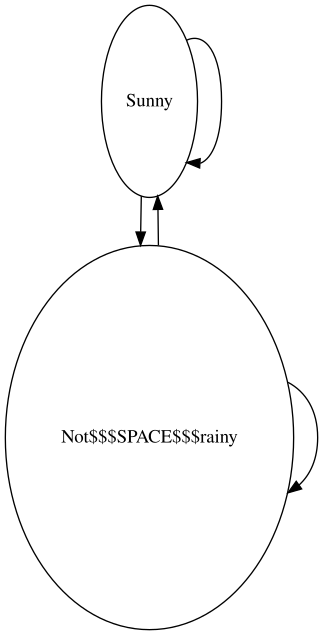
\includegraphics[]{create_bundled_vertices_markov_chain.png}
  \caption{
    .svg file created from the create\_bundled\_vertices\_markov\_chain function
    (algorithm \ref{lst:create_bundled_vertices_markov_chain}) 
    its .dot file, converted from .dot file to .svg 
    using algorithm \ref{lst:convert_dot_to_svg}
  }
  \label{fig:create_bundled_vertices_markov_chain.svg}
\end{figure}

%%%%%%%%%%%%%%%%%%%%%%%%%%%%%%%%%%%%%%%%%%%%%%%%%%%%%%%%%%%%%%%%%%%%%%%%%%%%%%%%
\section{Creating $K_{2}$ with bundled vertices}
\label{subsec:create_bundled_vertices_k2_graph}
%%%%%%%%%%%%%%%%%%%%%%%%%%%%%%%%%%%%%%%%%%%%%%%%%%%%%%%%%%%%%%%%%%%%%%%%%%%%%%%%

\subsection{Graph}

We reproduce the $K_{2}$ without properties of 
chapter \ref{subsec:create_k2_graph}, 
but with our bundled vertices instead, 
as show in figure \ref{fig:bundled_vertices_k2_graph}:

\begin{figure}
  \begin{tikzpicture}[->,>=stealth,shorten>=1pt,auto,node distance=4cm,semithick]
    \tikzstyle{every state}=[]
    \node[state] (A)              {Me,Myself,1.0,2.0};   
    \node[state] (B) [right of=A] {My computer,Not me,3.0,4.0};   
    \path (A) edge [] node {} (B); 
  \end{tikzpicture}
  \caption{
    $K_{2}$: a fully connected graph with two bundled vertices
  }
  \label{fig:bundled_vertices_k2_graph}
\end{figure}

\subsection{Function to create such a graph}

\lstinputlisting[
  caption = Creating $K_{2}$ as depicted in figure \ref{fig:bundled_vertices_k2_graph},
  label = lst:create_bundled_vertices_k2_graph
]{create_bundled_vertices_k2_graph.impl}
\index{Create bundled vertices K2 graph}

Most of the code is a slight modification of the 
\verb;create_k2_graph; function 
(algorithm \ref{lst:create_k2_graph}).
In the end, (references to) the \verb;my_bundled_vertices; 
are obtained and set with two bundled \verb;my_bundled_vertex; objects.

\subsection{Creating such a graph}

Demo:

\lstinputlisting[
  caption = Demo of the create\_bundled\_vertices\_k2\_graph function (algorithm \ref{lst:create_bundled_vertices_k2_graph}),
  label = lst:create_bundled_vertices_k2_graph_demo
]{create_bundled_vertices_k2_graph_demo.impl}

\subsection{The .dot file produced}

\lstinputlisting[
  caption = .dot file created from the create\_bundled\_vertices\_k2\_graph function (algorithm \ref{lst:create_bundled_vertices_k2_graph}) converted from graph to .dot file using algorithm \ref{lst:save_graph_to_dot},
  label = lst:create_bundled_vertices_k2_graph.dot-1
]{create_bundled_vertices_k2_graph.dot}

\subsection{The .svg file produced}

\begin{figure}[!htbp]
  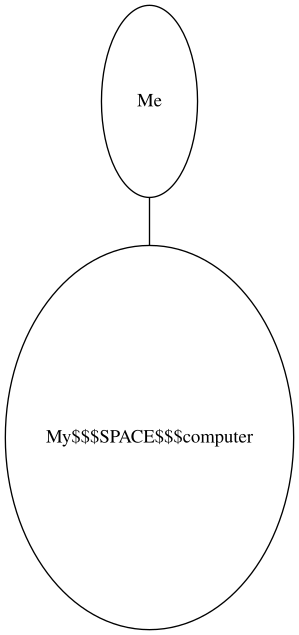
\includegraphics[]{create_bundled_vertices_k2_graph.png}
  \caption{
    .svg file created from the create\_bundled\_vertices\_k2\_graph function 
    (algorithm \ref{lst:create_bundled_vertices_k2_graph}) its .dot file, 
    converted from .dot file to .svg 
    using algorithm \ref{lst:convert_dot_to_svg}
  }
  \label{fig:create_bundled_vertices_k2_graph.svg}
\end{figure}


%%%%%%%%%%%%%%%%%%%%%%%%%%%%%%%%%%%%%%%%%%%%%%%%%%%%%%%%%%%%%%%%%%%%%%%%%%%%%%%%%
\chapter{Working on graphs with bundled vertices}
\label{sec:Working-on-graphs-with-bundled-vertices}
%%%%%%%%%%%%%%%%%%%%%%%%%%%%%%%%%%%%%%%%%%%%%%%%%%%%%%%%%%%%%%%%%%%%%%%%%%%%%%%%

When using graphs with bundled vertices, their state gives a way to find
a vertex and working with it.
This chapter shows some basic operations on graphs with bundled vertices.

\begin{itemize}
  \item Check if there exists a vertex with a certain \verb;my_bundled_vertex;: 
    chapter \ref{subsec:has_bundled_vertex_with_my_vertex}
  \item Find a vertex with a certain \verb;my_bundled_vertex;: 
    chapter \ref{subsec:find_bundled_vertex_with_my_vertex}
  \item Get a vertex its \verb;my_bundled_vertex; from its vertex descriptor: 
    chapter \ref{subsec:get_bundled_vertex_my_vertex}
  \item Set a vertex its \verb;my_bundled_vertex; using its vertex descriptor: 
    chapter \ref{subsec:set_bundled_vertex_my_vertex}
  \item Setting all vertices their \verb;my_bundled_vertex;-es: 
    chapter \ref{subsec:set_bundled_vertex_my_vertexes}
  \item Storing an directed/undirected graph with bundled vertices as a .dot file: 
    chapter \ref{subsec:save_bundled_vertices_graph_to_dot}
  \item Loading a directed graph with bundled vertices from a .dot file: 
    chapter \ref{subsec:load_directed_bundled_vertices_graph_from_dot}
  \item Loading an undirected directed graph with bundled vertices from a .dot file:
    chapter \ref{subsec:load_undirected_bundled_vertices_graph_from_dot}
\end{itemize}



%%%%%%%%%%%%%%%%%%%%%%%%%%%%%%%%%%%%%%%%%%%%%%%%%%%%%%%%%%%%%%%%%%%%%%%%%%%%%%%%%
\chapter{Building graphs with bundled edges and vertices}
%%%%%%%%%%%%%%%%%%%%%%%%%%%%%%%%%%%%%%%%%%%%%%%%%%%%%%%%%%%%%%%%%%%%%%%%%%%%%%%%

Up until now, the graphs created have had only bundled vertices.
In this chapter, graphs will be created, in which both the edges and vertices
have a bundled \verb;my_bundled_edge; and \verb;my_bundled_edge; type
\footnote{I do not intend to be original in naming my data types}.

\begin{itemize}
  \item An empty directed graph that allows for bundled edges and vertices: 
    see chapter \ref{subsec:create_empty_directed_bundled_edges_and_vertices_graph}
  \item An empty undirected graph that allows for bundled edges and vertices: 
    see chapter \ref{subsec:create_empty_undirected_bundled_edges_and_vertices_graph}
  \item A two-state Markov chain with bundled edges and vertices: 
    see chapter \ref{subsec:create_bundled_edges_and_vertices_markov_chain}
  \item $K_{3}$ with bundled edges and vertices: 
    see chapter \ref{subsec:create_bundled_edges_and_vertices_k3}
\end{itemize}

In the process, some basic (sometimes bordering trivial) functions are shown:

\begin{itemize}
  \item Creating the \verb;my_bundled_edge; class: 
    see chapter \ref{subsec:my_bundled_edge}
  \item Adding a bundled \verb;my_bundled_edge;: 
    see chapter \ref{subsec:add_bundled_edge}
\end{itemize}

These functions are mostly there for completion and showing which data types
are used.

%%%%%%%%%%%%%%%%%%%%%%%%%%%%%%%%%%%%%%%%%%%%%%%%%%%%%%%%%%%%%%%%%%%%%%%%%%%%%%%%
\section{Creating the bundled edge class}
\label{subsec:my_bundled_edge}
%%%%%%%%%%%%%%%%%%%%%%%%%%%%%%%%%%%%%%%%%%%%%%%%%%%%%%%%%%%%%%%%%%%%%%%%%%%%%%%%

In this example, I create a \verb;my_bundled_edge; class.
Here I will show the header file of it, as the implementation of it is
not important yet.

\lstinputlisting[
  caption = Declaration of my\_bundled\_edge,
  label = lst:my_bundled_edge_h
]{my_bundled_edge.impl}
\index{my\_bundled\_edge}
\index{my\_bundled\_edge.h}
\index{my\_bundled\_edge declaration}
\index{Declaration, my\_bundled\_edge}

\verb;my_bundled_edge; is a class that has multiple properties: 
two doubles \verb;m_width; 
(\verb;m_; \index{m\_} stands for member \index{member}) 
and \verb;m_height;, 
and two std::strings \verb;m_name; and \verb;m_description;.
\verb;my_bundled_edge; is copyable, 
but cannot trivially be converted to a \verb;std::string;. 
\verb;my_bundled_edge; is comparable for equality 
(that is, operator== is defined).
\verb;my_bundled_edge; does not have to have the stream operators defined for
file I/O, as this goes via the public member variables.

%%%%%%%%%%%%%%%%%%%%%%%%%%%%%%%%%%%%%%%%%%%%%%%%%%%%%%%%%%%%%%%%%%%%%%%%%%%%%%%%
\section{Create an empty directed graph with bundled edges and vertices}
\label{subsec:create_empty_directed_bundled_edges_and_vertices_graph}
%%%%%%%%%%%%%%%%%%%%%%%%%%%%%%%%%%%%%%%%%%%%%%%%%%%%%%%%%%%%%%%%%%%%%%%%%%%%%%%%

\lstinputlisting[
  caption = Creating an empty directed graph with bundled edges and vertices,
  label = lst:create_empty_directed_bundled_edges_and_vertices_graph
]{create_empty_directed_bundled_edges_and_vertices_graph.impl}
\index{Create empty directed bundled edges and vertices graph}

This code is very similar to the code described in chapter 
\ref{subsec:create_empty_directed_bundled_vertices_graph}, 
except that there is a new, fifth template argument:

\begin{verbatim}
boost::property<boost::edge_bundled_type_t, my_edge>
\end{verbatim}
\index{boost::property}
\index{boost::edge\_bundled\_type\_t}
\index{my\_edge}

This can be read as: 
\begin{quote}
edges have the property \verb;boost::edge_bundled_type_t;, 
which is of data type \verb;my_bundled_edge;
\end{quote}

Or simply: 

\begin{quote}
edges have a bundled type called my\_bundled\_edge
\end{quote}

Demo:

\lstinputlisting[
  caption = Demonstration of the create\_empty\_directed\_bundled\_edges\_and\_vertices\_graph function,
  label = lst:create_empty_directed_bundled_edges_and_vertices_graph_demo
]{create_empty_directed_bundled_edges_and_vertices_graph_demo.impl}

%%%%%%%%%%%%%%%%%%%%%%%%%%%%%%%%%%%%%%%%%%%%%%%%%%%%%%%%%%%%%%%%%%%%%%%%%%%%%%%%
\section{Create an empty undirected graph with bundled edges and vertices}
\label{subsec:create_empty_undirected_bundled_edges_and_vertices_graph}
%%%%%%%%%%%%%%%%%%%%%%%%%%%%%%%%%%%%%%%%%%%%%%%%%%%%%%%%%%%%%%%%%%%%%%%%%%%%%%%%

\lstinputlisting[
  caption = Creating an empty undirected graph with bundled edges and vertices,
  label = lst:create_empty_undirected_bundled_edges_and_vertices_graph
]{create_empty_undirected_bundled_edges_and_vertices_graph.impl}
\index{Create empty undirected bundled edges and vertices graph}

This code is very similar to the code described in chapter 
\ref{subsec:create_empty_directed_bundled_edges_and_vertices_graph}, 
except that the directness (the third template argument) is undirected
 (due to the boost::undirectedS \index{boost::undirectedS}).

Demo:

\lstinputlisting[
  caption = Demonstration of the create\_empty\_undirected\_bundled\_edges\_and\_vertices\_graph function,
  label = lst:create_empty_undirected_bundled_edges_and_vertices_graph_demo
]{create_empty_undirected_bundled_edges_and_vertices_graph_demo.impl}

%%%%%%%%%%%%%%%%%%%%%%%%%%%%%%%%%%%%%%%%%%%%%%%%%%%%%%%%%%%%%%%%%%%%%%%%%%%%%%%%
\section{Add a bundled edge}
\label{subsec:add_bundled_edge}
%%%%%%%%%%%%%%%%%%%%%%%%%%%%%%%%%%%%%%%%%%%%%%%%%%%%%%%%%%%%%%%%%%%%%%%%%%%%%%%%

Adding a bundled edge is very similar to adding an edge 
without properties (chapter \ref{subsec:add_edge}).

\lstinputlisting[
  caption = Add a bundled edge,
  label = lst:add_bundled_edge
]{add_bundled_edge.impl}
\index{Add bundled edge}

When having added a new (abstract) edge to the graph, the edge descriptor
is used to set the \verb;my_edge; in the graph.

Here is the demo:

\lstinputlisting[
  caption = Demo of add\_bundled\_edge,
  label = lst:add_bundled_edge_demo
]{add_bundled_edge_demo.impl}

%%%%%%%%%%%%%%%%%%%%%%%%%%%%%%%%%%%%%%%%%%%%%%%%%%%%%%%%%%%%%%%%%%%%%%%%%%%%%%%%
\section{Getting the bundled edges my\_edges}
\label{subsec:get_bundled_edge_my_edges}
%%%%%%%%%%%%%%%%%%%%%%%%%%%%%%%%%%%%%%%%%%%%%%%%%%%%%%%%%%%%%%%%%%%%%%%%%%%%%%%%

When the edges of a graph are \verb;my_bundled_edge; objects, 
one can extract these all as such:

\lstinputlisting[
  caption = Get the edges' my\_bundled\_edges,
  label = lst:get_bundled_edge_my_edges
]{get_my_bundled_edges.impl}
\index{Get edge my\_bundled\_edges}

The \verb;my_bundled_edge; object associated with the edges are obtained from
the graph its \verb;property_map\verb; and then put into a 
\verb;std::vector; \index{std::vector}.

Note: the order of the \verb;my_bundled_edge; objects may be different after saving
and loading.

When trying to get the edges' \verb;my_bundled_edge; objects from a graph without
bundled edges objects associated, you will get the error 
\verb;formed reference to void; (see chapter \ref{subsec:formed_reference_to_void}).

%%%%%%%%%%%%%%%%%%%%%%%%%%%%%%%%%%%%%%%%%%%%%%%%%%%%%%%%%%%%%%%%%%%%%%%%%%%%%%%%
\section{Creating a Markov-chain with bundled edges and vertices}
\label{subsec:create_bundled_edges_and_vertices_markov_chain}
%%%%%%%%%%%%%%%%%%%%%%%%%%%%%%%%%%%%%%%%%%%%%%%%%%%%%%%%%%%%%%%%%%%%%%%%%%%%%%%%

\subsection{Graph}

Figure \ref{fig:bundled_edges_and_vertices_markov_chain}
shows the graph that will be reproduced:

\begin{figure}
  \begin{tikzpicture}[->,>=stealth',auto,node distance=9cm, semithick]
    \tikzstyle{every state}=[]
    \node[state] (A) 
      {Stable,Right, 1.0, 2.0};   
    \node[state] (B) [right of=A] 
      {Not unstable,Not left, 3.0, 4.0}
    ;   
    \path (A) edge [loop above] node {Red,Heat,1,2} (A)
          (A) edge [bend  left] node {Orange,Lose heat,3,4} (B)
          (B) edge [bend  left] node {Yellow cold,Heat,4,5} (A)
          (B) edge [loop above] node {Green cols,Stay cool,6,7} (B); 
  \end{tikzpicture}
  \caption{
    A two-state Markov chain where the edges and vertices have bundled properties.
    The edges' and vertices' properties are nonsensical
  }
  \label{fig:bundled_edges_and_vertices_markov_chain}
\end{figure}

\subsection{Function to create such a graph}

Here is the code creating a two-state Markov chain with bundled edges and
vertices:

\lstinputlisting[
  caption = Creating the two-state Markov chain as depicted in figure \ref{fig:bundled_edges_and_vertices_markov_chain},
  label = lst:create_bundled_edges_and_vertices_markov_chain
]{create_bundled_edges_and_vertices_markov_chain.impl}
\index{Create bundled edges and vertices Markov chain}

\subsection{Creating such a graph}

Here is the demo:

\lstinputlisting[
  caption = Demo of the create\_bundled\_edges\_and\_vertices\_markov\_chain function (algorithm \ref{lst:create_bundled_edges_and_vertices_markov_chain}),
  label = lst:create_bundled_edges_and_vertices_markov_chain_demo
]{create_bundled_edges_and_vertices_markov_chain_demo.impl}

\subsection{The .dot file produced}

\lstinputlisting[
  caption = .dot file created from the create\_bundled\_edges\_and\_vertices\_markov\_chain function (algorithm \ref{lst:create_bundled_edges_and_vertices_markov_chain}) converted from graph to .dot file using algorithm \ref{lst:save_graph_to_dot},
  label = lst:create_bundled_edges_and_vertices_markov_chain.dot
]{create_bundled_edges_and_vertices_markov_chain.dot}

\subsection{The .svg file produced}

\begin{figure}[!htbp]
  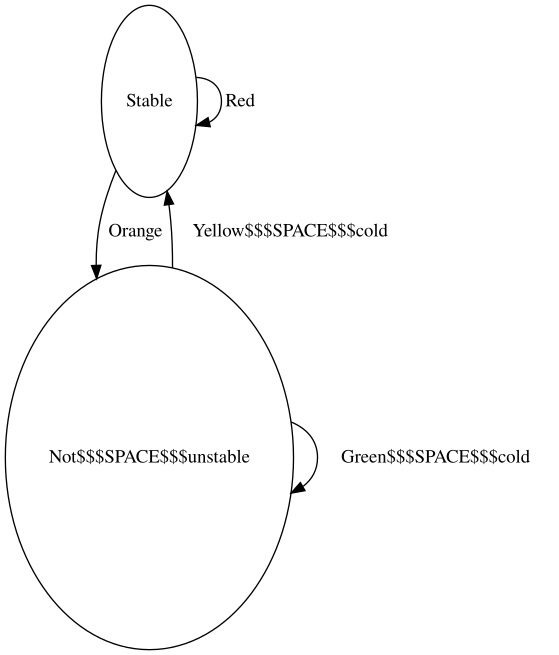
\includegraphics[]{create_bundled_edges_and_vertices_markov_chain.png}
  \caption{
    .svg file created from the create\_bundled\_edges\_and\_vertices\_markov\_chain function 
    (algorithm  \ref{lst:create_bundled_vertices_markov_chain}) 
    its .dot file converted from .dot file to .svg using algorithm 
    \ref{lst:convert_dot_to_svg}
  }
  \label{fig:create_bundled_edges_and_vertices_markov_chain.svg}
\end{figure}

%%%%%%%%%%%%%%%%%%%%%%%%%%%%%%%%%%%%%%%%%%%%%%%%%%%%%%%%%%%%%%%%%%%%%%%%%%%%%%%%
\section{Creating $K_{3}$  with bundled edges and vertices}
\label{subsec:create_bundled_edges_and_vertices_k3}
%%%%%%%%%%%%%%%%%%%%%%%%%%%%%%%%%%%%%%%%%%%%%%%%%%%%%%%%%%%%%%%%%%%%%%%%%%%%%%%%

Instead of using edges with a name, or other properties, here we use a bundled
edge class called \verb;my_bundled_edge;.

\subsection{Graph}

We reproduce the $K_{3}$ without properties of chapter 
\ref{subsec:create_k3_graph}, but with our bundled edges and vertices instead:

\begin{figure}
  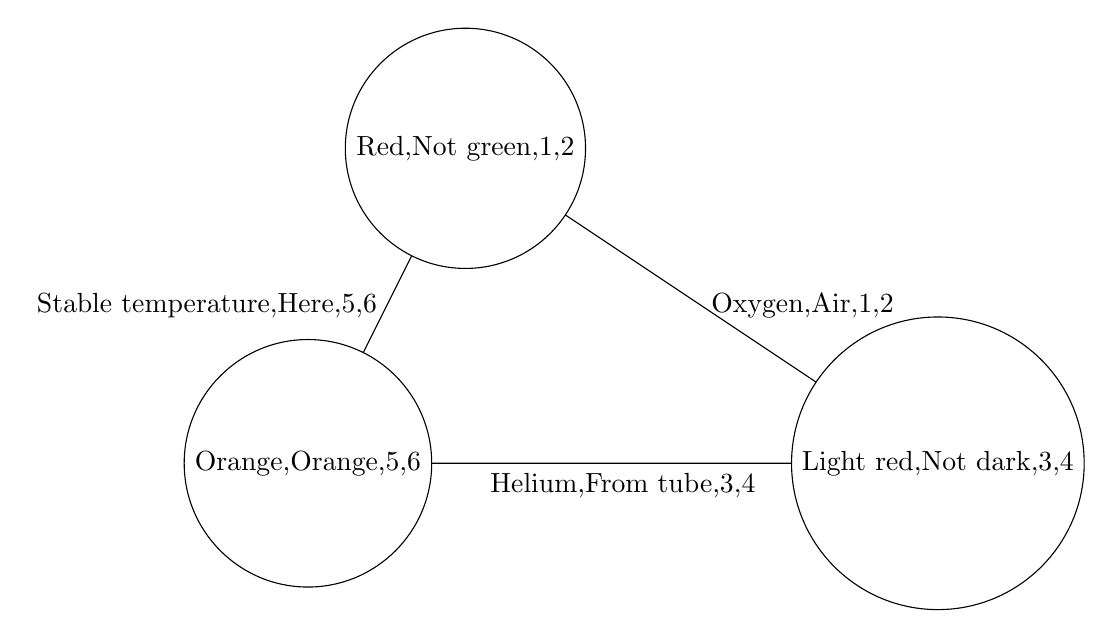
\begin{tikzpicture}
    \draw[] 
      (2,4) node[draw=black,fill=white,shape=circle,text=black] {Red,Not green,1,2}
       -- (5,2) node[anchor=west] {Oxygen,Air,1,2} 
       -- (8,0) node[draw=black,fill=white,shape=circle,text=black] {Light red,Not dark,3,4} 
       -- (4,0) node[anchor=north] {Helium,From tube,3,4} 
       -- (0,0) node[draw=black,fill=white,shape=circle,text=black] {Orange,Orange,5,6} 
       -- (1,2) node[anchor=east] {Stable temperature,Here,5,6} 
       -- (2,4)
    ;
  \end{tikzpicture}
  \caption{$K_{3}$: a fully connected graph with three bundled edges and vertices }
  \label{fig:create_bundled_edges_and_vertices_k3}
\end{figure}

\subsection{Function to create such a graph}

\lstinputlisting[
  caption = Creating $K_{3}$ as depicted in figure \ref{fig:create_bundled_edges_and_vertices_k3},
  label = lst:create_bundled_edges_and_vertices_k3_graph
]{create_bundled_edges_and_vertices_k3_graph.impl}
\index{Create bundled edges and vertices K3 graph}

Most of the code is a slight modification of algorithm 
\ref{lst:create_k3_graph}.
In the end, the \verb;my_edges; and \verb;my_vertices; are obtained as the graph its
\verb;property_map; and set with the \verb;my_bundled_edge; 
and \verb;my_bundled_vertex; objects.

\subsection{Creating such a graph

Here is the demo:

\lstinputlisting[
  caption = Demo of the create\_bundled\_edges\_and\_vertices\_k3\_graph function (algorithm \ref{lst:create_bundled_edges_and_vertices_k3_graph}),
  label = lst:create_bundled_edges_and_vertices_k3_graph_demo
]{create_bundled_edges_and_vertices_k3_graph_demo.impl}

\subsection{The .dot file produced}

\lstinputlisting[
  caption = .dot file created from the create\_bundled\_edges\_and\_vertices\_markov\_chain function (algorithm \ref{lst:create_bundled_edges_and_vertices_k3_graph}) converted from graph to .dot file using algorithm \ref{lst:save_graph_to_dot},
  label = lst:create_bundled_edges_and_vertices_k3_graph.dot
]{create_bundled_edges_and_vertices_k3_graph.dot}

\subsection{The .svg file produced}

\begin{figure}[!htbp]
  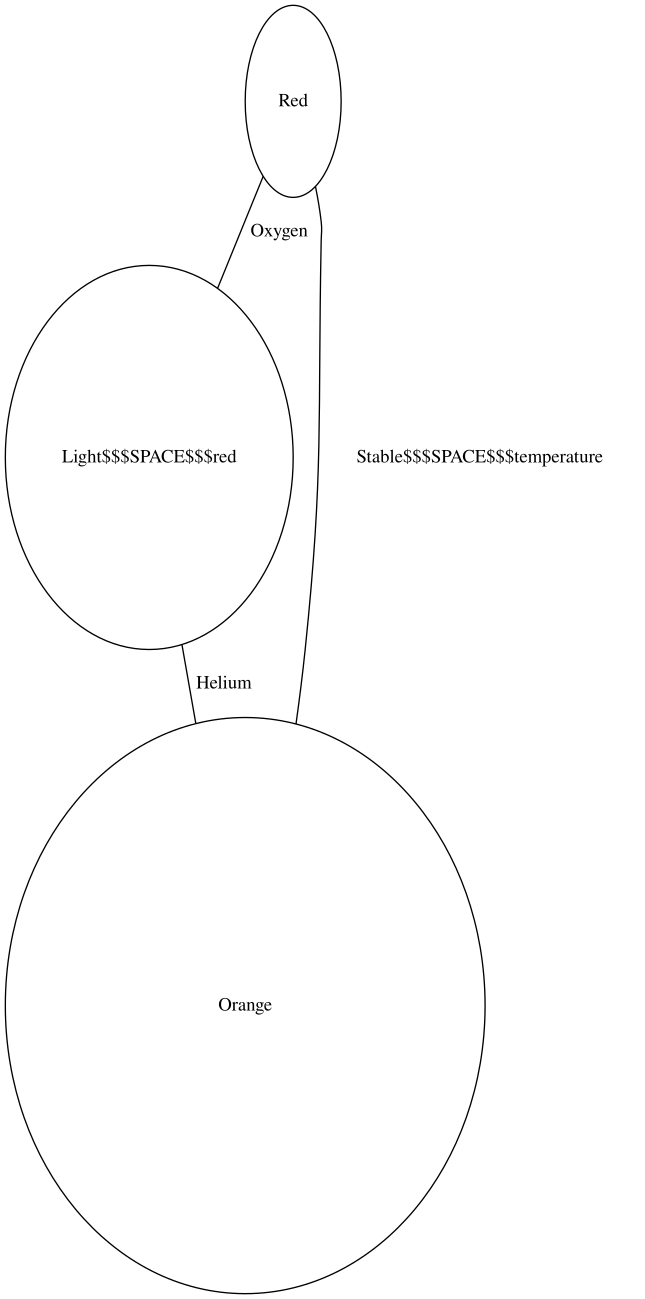
\includegraphics[]{create_bundled_edges_and_vertices_k3_graph.png}
  \caption{
    .svg file created from the create\_bundled\_edges\_and\_vertices\_k3\_graph function
    (algorithm \ref{lst:create_bundled_vertices_markov_chain}) 
    its .dot file, converted from .dot file to .svg using algorithm 
    \ref{lst:convert_dot_to_svg}
  }
  \label{fig:create_bundled_edges_and_vertices_k3_graph.svg}
\end{figure}


%%%%%%%%%%%%%%%%%%%%%%%%%%%%%%%%%%%%%%%%%%%%%%%%%%%%%%%%%%%%%%%%%%%%%%%%%%%%%%%%%
\chapter{Working on graphs with bundled edges and vertices}
%%%%%%%%%%%%%%%%%%%%%%%%%%%%%%%%%%%%%%%%%%%%%%%%%%%%%%%%%%%%%%%%%%%%%%%%%%%%%%%%

%%%%%%%%%%%%%%%%%%%%%%%%%%%%%%%%%%%%%%%%%%%%%%%%%%%%%%%%%%%%%%%%%%%%%%%%%%%%%%%%
\section{Has a my\_bundled\_edge}
\label{subsec:has_bundled_edge_with_my_edge}
%%%%%%%%%%%%%%%%%%%%%%%%%%%%%%%%%%%%%%%%%%%%%%%%%%%%%%%%%%%%%%%%%%%%%%%%%%%%%%%%

Before modifying our edges, let's first determine if we can find an edge
by its bundled type (\verb;my_bundled_edge;) in a graph.
After obtaining a my\_bundled\_edge map, 
we obtain the edge iterators, dereference these to obtain 
the edge descriptors and then compare each edge its my\_bundled\_edge 
with the one desired.

\lstinputlisting[
  caption = Find if there is a bundled edge with a certain my\_bundled\_edge,
  label = lst:has_bundled_edge_with_my_edge
]{has_bundled_edge_with_my_edge.impl}
\index{Has bundled edge with my_bundled_edge}

This function can be demonstrated as in algorithm 
\ref{lst:has_bundled_edge_with_my_edge_demo}, 
where a certain \verb;my_bundled_edge; cannot be found in an empty graph.
After adding the desired my\_bundled\_edge, it is found.

\lstinputlisting[
  caption = Demonstration of the has\_bundled\_edge\_with\_my\_edge function,
  label = lst:has_bundled_edge_with_my_edge_demo
]{has_bundled_edge_with_my_edge_demo.impl}

Note that this function only finds if there is at least one edge with that
my\_bundled\_edge: it does not tell how many edges with that my_bundled_edge
exist in the graph.

%%%%%%%%%%%%%%%%%%%%%%%%%%%%%%%%%%%%%%%%%%%%%%%%%%%%%%%%%%%%%%%%%%%%%%%%%%%%%%%%
\section{Find a my\_bundled\_edge}
\label{subsec:find_first_bundled_edge_with_my_edge}
%%%%%%%%%%%%%%%%%%%%%%%%%%%%%%%%%%%%%%%%%%%%%%%%%%%%%%%%%%%%%%%%%%%%%%%%%%%%%%%%

Where STL functions work with iterators, here we obtain an edge descriptor
(see chapter \ref{subsec:Edge-descriptors}) 
to obtain a handle to the desired edge.
Listing \ref{lst:find_first_bundled_edge_with_my_edge}
shows how to obtain an edge descriptor to the first edge found with a specific
my_bundled_edge value.

\lstinputlisting[
  caption = Find the first bundled edge with a certain my\_bundled\_edge,
  label = lst:find_first_bundled_edge_with_my_edge
]{find_first_bundled_edge_with_my_edge.impl}
\index{Find first bundled edge with my_bundled_edge}

With the edge descriptor obtained, one can read and modify the edge and
the vertices surrounding it.
Listing \ref{lst:find_first_bundled_edge_with_my_edge_demo}
shows some examples of how to do so.

\lstinputlisting[
  caption = Demonstration of the find\_first\_bundled\_edge\_with\_my\_edge function,
  label = lst:find_first_bundled_edge_with_my_edge_demo
]{find_first_bundled_edge_with_my_edge_demo.impl}

%%%%%%%%%%%%%%%%%%%%%%%%%%%%%%%%%%%%%%%%%%%%%%%%%%%%%%%%%%%%%%%%%%%%%%%%%%%%%%%%
\section{Get an edge its my\_bundled\_edge}
\label{subsec:get_bundled_edge_my_edge}
%%%%%%%%%%%%%%%%%%%%%%%%%%%%%%%%%%%%%%%%%%%%%%%%%%%%%%%%%%%%%%%%%%%%%%%%%%%%%%%%

To obtain the my\_bundled\_edge from an edge descriptor, one needs to pull
out the my\_bundled_edges map and then look up the my\_edge of interest.

\lstinputlisting[
  caption = Get a vertex its my\_bundled\_vertex from its vertex descriptor,
  label = lst:get_bundled_edge_my_edge
]{get_my_bundled_edge.impl}
\index{Get my_bundled_edge}

To use \verb;get_my_bundled_edge;, 
one first needs to obtain an edge descriptor.
Listing \ref{lst:get_bundled_edge_my_edge_demo} shows a simple example.

\lstinputlisting[
  caption = Demonstration if the get\_my\_bundled\_edge function,
  label = lst:get_bundled_edge_my_edge_demo
]{get_my_bundled_edge_demo.impl}

%%%%%%%%%%%%%%%%%%%%%%%%%%%%%%%%%%%%%%%%%%%%%%%%%%%%%%%%%%%%%%%%%%%%%%%%%%%%%%%%
\section{Set an edge its my\_bundled\_edge}
\label{subsec:set_bundled_edge_my_edge}
%%%%%%%%%%%%%%%%%%%%%%%%%%%%%%%%%%%%%%%%%%%%%%%%%%%%%%%%%%%%%%%%%%%%%%%%%%%%%%%%

If you know how to get the my_bundled_edge from an edge descriptor, 
setting it is just as easy, as shown in algorithm \ref{lst:set_bundled_edge_my_edge}.

\lstinputlisting[
  caption = Set a bundled edge its my\_bundled\_edge from its edge descriptor,
  label = lst:set_bundled_edge_my_edge
]{set_my_bundled_edge.impl}
\index{Set bundled edge my_bundled_edge}

To use \verb;set_bundled_edge_my_edge;, 
one first needs to obtain an edge descriptor.
Listing \ref{lst:set_bundled_edge_my_edge_demo}
shows a simple example.

\lstinputlisting[
  caption = Demonstration if the set\_bundled\_edge\_my\_edge function,
  label = lst:set_bundled_edge_my_edge_demo
]{set_my_bundled_edge_demo.impl}

%%%%%%%%%%%%%%%%%%%%%%%%%%%%%%%%%%%%%%%%%%%%%%%%%%%%%%%%%%%%%%%%%%%%%%%%%%%%%%%%
\section{Storing a graph with bundled edges and vertices as a .dot}
\label{subsec:save_bundled_edges_and_vertices_graph_to_dot}
\index{Save graph with bundled edges and vertices as .dot}
\index{Create .dot from graph with bundled edges and vertices}
%%%%%%%%%%%%%%%%%%%%%%%%%%%%%%%%%%%%%%%%%%%%%%%%%%%%%%%%%%%%%%%%%%%%%%%%%%%%%%%%

If you used the \verb;create_bundled_edges_and_vertices_k3_graph; 
function (algorithm \ref{lst:create_bundled_edges_and_vertices_k3_graph}) 
to produce a $K_{3}$ graph with edges and vertices 
associated with my\_bundled\_edge and my\_bundled\_vertex objects, 
you can store these my\_bundled\_edges and my\_bundled\_vertex-es
additionally with algorithm \ref{lst:save_bundled_edges_and_vertices_graph_to_dot}:

\lstinputlisting[
  caption = Storing a graph with bundled edges and vertices as a .dot file,
  label = lst:save_bundled_edges_and_vertices_graph_to_dot
]{save_bundled_edges_and_vertices_graph_to_dot.impl}
\index{Save bundled edges and vertices graph to dot}


%%%%%%%%%%%%%%%%%%%%%%%%%%%%%%%%%%%%%%%%%%%%%%%%%%%%%%%%%%%%%%%%%%%%%%%%%%%%%%%%%
\chapter{Building graphs with a graph name}
\label{sec:Building-graphs-with-a-graph-name}
%%%%%%%%%%%%%%%%%%%%%%%%%%%%%%%%%%%%%%%%%%%%%%%%%%%%%%%%%%%%%%%%%%%%%%%%%%%%%%%%

Up until now, the graphs created have had no properties themselves.
Sure, the edges and vertices have had properties, but the graph itself
has had none.
Until now.

In this chapter, graphs will be created with a graph name of type std::string

\begin{itemize}
  \item An empty directed graph with a graph name: 
    see chapter 
  \item An empty undirected graph with a graph name: 
    see chapter 
  \item A two-state Markov chain with a graph name: 
    see chapter
  \item $K_{3}$ with a graph name: 
   see chapter 
\end{itemize}

In the process, some basic (sometimes bordering trivial) functions are shown:

\begin{itemize}
  \item Getting a graph its name: 
    see chapter 
  \item Setting a graph its name: 
    see chapter
\end{itemize}

%%%%%%%%%%%%%%%%%%%%%%%%%%%%%%%%%%%%%%%%%%%%%%%%%%%%%%%%%%%%%%%%%%%%%%%%%%%%%%%%
\section{Create an empty directed graph with a graph name property}
\label{subsec:create_empty_directed_graph_with_graph_name}
%%%%%%%%%%%%%%%%%%%%%%%%%%%%%%%%%%%%%%%%%%%%%%%%%%%%%%%%%%%%%%%%%%%%%%%%%%%%%%%%

Listing 
\ref{lst:create_empty_directed_graph_with_graph_name}
shows the function to create an empty directed graph with a graph name.

\lstinputlisting[
  caption = Creating an empty directed graph with a graph name,
  label = lst:create_empty_directed_graph_with_graph_name
]{create_empty_directed_graph_with_graph_name.impl}
\index{Create empty directed graph with graph name}

This \verb;boost::adjacency_list; is of the following type:

\begin{itemize}
  \item the first \verb;boost::vecS; \index{boost::vecS}: 
    select (that is what the \verb;S; \index{S} means) 
    that out edges are stored in a std::vector.
    This is the default way.
  \item the second \verb;boost::vecS; \index{boost::vecS}: 
    select that the graph vertices are stored in a std::vector.
    This is the default way.
  \item \verb;boost::directedS; \index{boost::directedS}: 
    select that the graph is directed.
    This is the default selectedness
  \item the first \verb;boost::no_property; \index{boost::no\_property}: 
    the vertices have no properties.
    This is the default (non-)property
  \item the second \verb;boost::no_property; \index{boost::no\_property}: 
    the vertices have no properties.
    This is the default (non-)property
  \item
    \verb;boost::property<boost::graph_name_t, std::string>; 
    \index{boost::property}
    \index{boost::graph\_name\_t}: 
    the graph itself has a single property: 
    its \verb;boost::graph_name; \index{boost::graph\_name} has type std::string
\end{itemize}

Listing 
\ref{lst:create_empty_directed_graph_with_graph_name_demo}
demonstrates the \verb;create_empty_directed_graph_with_graph_name; function.

\lstinputlisting[
  caption = Demonstration of create\_empty\_directed\_graph\_with\_graph\_name,
  label = lst:create_empty_directed_graph_with_graph_name_demo
]{create_empty_directed_graph_with_graph_name_demo.impl}

%%%%%%%%%%%%%%%%%%%%%%%%%%%%%%%%%%%%%%%%%%%%%%%%%%%%%%%%%%%%%%%%%%%%%%%%%%%%%%%%
\section{Create an empty undirected graph with a graph name property}
\label{subsec:create_empty_undirected_graph_with_graph_name}
%%%%%%%%%%%%%%%%%%%%%%%%%%%%%%%%%%%%%%%%%%%%%%%%%%%%%%%%%%%%%%%%%%%%%%%%%%%%%%%%

Listing 
\ref{lst:create_empty_undirected_graph_with_graph_name}
shows the function to create an empty undirected graph with a graph name.

\lstinputlisting[
  caption = Creating an empty undirected graph with a graph name,
  label = lst:create_empty_undirected_graph_with_graph_name
]{create_empty_undirected_graph_with_graph_name.impl}
\index{Create empty undirected graph with graph name}

This code is very similar to the code described in chapter 
\ref{lst:create_empty_directed_graph_with_graph_name}, 
except that the directness (the third template argument) is undirected
(due to the boost::undirectedS \index{boost::undirectedS}).

Listing \ref{lst:create_empty_undirected_graph_with_graph_name_demo}
demonstrates the \verb;create_empty_undirected_graph_with_graph_name; function.

\lstinputlisting[
  caption = Demonstration of create\_empty\_undirected\_graph\_with\_graph\_name,
  label = lst:create_empty_undirected_graph_with_graph_name_demo
]{create_empty_undirected_graph_with_graph_name_demo.impl}

%%%%%%%%%%%%%%%%%%%%%%%%%%%%%%%%%%%%%%%%%%%%%%%%%%%%%%%%%%%%%%%%%%%%%%%%%%%%%%%%
\section{Get a graph its name property}
\label{subsec:get_graph_name}
%%%%%%%%%%%%%%%%%%%%%%%%%%%%%%%%%%%%%%%%%%%%%%%%%%%%%%%%%%%%%%%%%%%%%%%%%%%%%%%%

\lstinputlisting[
  caption = Get a graph its name,
  label = lst:get_graph_name
]{get_graph_name.impl}
\index{Get graph name}

Listing \ref{lst:get_graph_name_demo}
demonstrates the \verb;get_graph_name; function.

\lstinputlisting[
  caption = Demonstration of get\_graph\_name,
  label = lst:get_graph_name_demo
]{get_graph_name_demo.impl}


%%%%%%%%%%%%%%%%%%%%%%%%%%%%%%%%%%%%%%%%%%%%%%%%%%%%%%%%%%%%%%%%%%%%%%%%%%%%%%%%%
\chapter{Working on graphs with a graph name}
%%%%%%%%%%%%%%%%%%%%%%%%%%%%%%%%%%%%%%%%%%%%%%%%%%%%%%%%%%%%%%%%%%%%%%%%%%%%%%%%

Working on graphs with a graph name text.

%%%%%%%%%%%%%%%%%%%%%%%%%%%%%%%%%%%%%%%%%%%%%%%%%%%%%%%%%%%%%%%%%%%%%%%%%%%%%%%%%
\chapter{Other graph functions}
%%%%%%%%%%%%%%%%%%%%%%%%%%%%%%%%%%%%%%%%%%%%%%%%%%%%%%%%%%%%%%%%%%%%%%%%%%%%%%%%

Other graph functions text.

%%%%%%%%%%%%%%%%%%%%%%%%%%%%%%%%%%%%%%%%%%%%%%%%%%%%%%%%%%%%%%%%%%%%%%%%%%%%%%%%%
\chapter{Misc functions}
%%%%%%%%%%%%%%%%%%%%%%%%%%%%%%%%%%%%%%%%%%%%%%%%%%%%%%%%%%%%%%%%%%%%%%%%%%%%%%%%

These are some function I needed for creating this tutorial.
Although they are not important for working with graphs, I used these heavily.
These functions may be compiler-dependent, platform-dependent and/or there
may be superior alternatives.
I just add them for completeness.

%%%%%%%%%%%%%%%%%%%%%%%%%%%%%%%%%%%%%%%%%%%%%%%%%%%%%%%%%%%%%%%%%%%%%%%%%%%%%%%%
\section{Getting a data type as a std::string}
\label{subsec:get_type_name}
%%%%%%%%%%%%%%%%%%%%%%%%%%%%%%%%%%%%%%%%%%%%%%%%%%%%%%%%%%%%%%%%%%%%%%%%%%%%%%%%

This function will only work under GCC.
I found this code at 
\url{
  http://stackoverflow.com/questions/1055452/c-get-name-of-type-in-template
}.
Thanks to \verb;m-dudley' 
(Stack Overflow user page at \url{http://stackoverflow.com/users/111327/m-dudley}).

\lstinputlisting[
  caption = Getting a data type its name as a std::string,
  label = lst:get_type_name
]{get_type_name.impl}
\index{Get type name}

%%%%%%%%%%%%%%%%%%%%%%%%%%%%%%%%%%%%%%%%%%%%%%%%%%%%%%%%%%%%%%%%%%%%%%%%%%%%%%%%
\section{Convert a .dot to .svg}
\label{subsec:convert_dot_to_svg}
%%%%%%%%%%%%%%%%%%%%%%%%%%%%%%%%%%%%%%%%%%%%%%%%%%%%%%%%%%%%%%%%%%%%%%%%%%%%%%%%

All illustrations in this tutorial are created by converting .dot to a .svg
(\verb;Scalable Vector Graphic;) file.
This function assumes the program \verb;dot; is installed, which is part of
Graphviz.

\lstinputlisting[
  caption = Convert a .dot file to a .svg,
  label = lst:convert_dot_to_svg
]{convert_dot_to_svg.impl}
\index{Convert dot to svg}

\verb;convert_dot_to_svg; makes a system call 
to the program \verb;dot; to convert
the .dot file to an .svg file.


%%%%%%%%%%%%%%%%%%%%%%%%%%%%%%%%%%%%%%%%%%%%%%%%%%%%%%%%%%%%%%%%%%%%%%%%%%%%%%%%%
\chapter{Errors}
%%%%%%%%%%%%%%%%%%%%%%%%%%%%%%%%%%%%%%%%%%%%%%%%%%%%%%%%%%%%%%%%%%%%%%%%%%%%%%%%

Some common errors.

%%%%%%%%%%%%%%%%%%%%%%%%%%%%%%%%%%%%%%%%%%%%%%%%%%%%%%%%%%%%%%%%%%%%%%%%%%%%%%%%
\section{Formed reference to void}
\label{subsec:formed_reference_to_void}
%%%%%%%%%%%%%%%%%%%%%%%%%%%%%%%%%%%%%%%%%%%%%%%%%%%%%%%%%%%%%%%%%%%%%%%%%%%%%%%%

This compile-time error occurs when you create a graph without a certain
 property, then subsequently reading that property, as in algorithm 
\ref{lst:formed_reference_to_void}: 

\lstinputlisting[
  caption = Creating the error 'formed reference to void',
  label = lst:formed_reference_to_void
]{formed_reference_to_void.impl}
\index{Formed reference to void}

In algorithm \ref{lst:formed_reference_to_void}
a graph is created with vertices of no properties.
Then the names of these vertices, which do not exists, are tried to be
read.
If you want to read the names of the vertices, supply a graph that has
this property.

%%%%%%%%%%%%%%%%%%%%%%%%%%%%%%%%%%%%%%%%%%%%%%%%%%%%%%%%%%%%%%%%%%%%%%%%%%%%%%%%
\section{No matching function for call to clear\_out\_edges}
\label{subsec:no_matching_function_for_call_to_clear_out_edges}
%%%%%%%%%%%%%%%%%%%%%%%%%%%%%%%%%%%%%%%%%%%%%%%%%%%%%%%%%%%%%%%%%%%%%%%%%%%%%%%%

This compile-time error occurs when you want to clear the outward edges
from a vertex in an undirected graph.

\lstinputlisting[
  caption = Creating the error 'no matching function for call to clear\_out\_edges',
  label = lst:no_matching_function_for_call_to_clear_out_edges
]{no_matching_function_for_call_to_clear_out_edges.impl}
\index{No matching function for call to clear\_out\_edges}

In algorithm 
\ref{lst:no_matching_function_for_call_to_clear_out_edges}
an undirected graph is created, a vertex descriptor is obtained, then its
out
edges are tried to be cleared. Either use a directed graph (which has out
edges), or use the \verb;boost::clear_vertex; function instead.

%%%%%%%%%%%%%%%%%%%%%%%%%%%%%%%%%%%%%%%%%%%%%%%%%%%%%%%%%%%%%%%%%%%%%%%%%%%%%%%%
\section{No matching function for call to \verb;clear_in_edges;}
\label{subsec:no_matching_function_for_call_to_clear_in_edges}
%%%%%%%%%%%%%%%%%%%%%%%%%%%%%%%%%%%%%%%%%%%%%%%%%%%%%%%%%%%%%%%%%%%%%%%%%%%%%%%%

See chapter \ref{subsec:no_matching_function_for_call_to_clear_out_edges}.

%%%%%%%%%%%%%%%%%%%%%%%%%%%%%%%%%%%%%%%%%%%%%%%%%%%%%%%%%%%%%%%%%%%%%%%%%%%%%%%%
\section{Undefined reference to boost::detail::graph::read_graphviz_new}
\label{subsec:undefined_reference_to_read_graphviz_new}
\index{read\_graphviz\_new}
\index{Undefined reference to read_graphviz\_new}
\index{read\_graphviz\_new, undefined reference}
%%%%%%%%%%%%%%%%%%%%%%%%%%%%%%%%%%%%%%%%%%%%%%%%%%%%%%%%%%%%%%%%%%%%%%%%%%%%%%%%

You will have to link \index{link}
against the Boost.Graph and Boost.Regex libraries.
In Qt Creator, this is achieved by adding these lines to your Qt Creator
project file:

\begin{verbatim}
LIBS += -lboost_graph -lboost_regex 
\end{verbatim}



%%%%%%%%%%%%%%%%%%%%%%%%%%%%%%%%%%%%%%%%%%%%%%%%%%%%%%%%%%%%%%%%%%%%%%%%%%%%%%%%
% Bibliography
%%%%%%%%%%%%%%%%%%%%%%%%%%%%%%%%%%%%%%%%%%%%%%%%%%%%%%%%%%%%%%%%%%%%%%%%%%%%%%%%
% Vancouver style
\bibliographystyle{unsrtnat}
% MEE style
%\bibliographystyle{mee}
\bibliography{boost_graph_cookbook_1}
%%%%%%%%%%%%%%%%%%%%%%%%%%%%%%%%%%%%%%%%%%%%%%%%%%%%%%%%%%%%%%%%%%%%%%%%%%%%%%%%

\newpage
\appendix

%%%%%%%%%%%%%%%%%%%%%%%%%%%%%%%%%%%%%%%%%%%%%%%%%%%%%%%%%%%%%%%%%%%%%%%%%%%%%%%%%
\chapter{Appendix}
%%%%%%%%%%%%%%%%%%%%%%%%%%%%%%%%%%%%%%%%%%%%%%%%%%%%%%%%%%%%%%%%%%%%%%%%%%%%%%%%

Appendix text.


\end{document}
